\documentclass{statsmsc}
\usepackage[
  bottom=0.3in,
  includefoot
]{geometry}
\title{Statistics Research Project Title}
\author{Jing Zhang}
\CID{06014353}
\supervisor{Daniel Mortlock}
%For today's date, use:
\date{\today}
\logoimg{}

% THIS IS WHERE NEW COMMANDS CAN BE DEFINED

% commands below only used in the proof; otherwise can be deleted
\newcommand{\consta}{a}
\newcommand{\X}{X}
\newcommand{\EE}[1]{ \mathrm{E} [ #1 ] }
\newcommand{\inparenth}[1]{\left( #1 \right)}
\usepackage{xcolor}
\usepackage{hyperref}
\hypersetup{
    colorlinks,
    linkcolor={blue!50!black},
    citecolor={blue!50!black},
    urlcolor={blue!50!black}
}
\usepackage{tikz}
\usetikzlibrary{positioning, arrows.meta, shapes.geometric}
\usepackage{enumitem}
\usepackage[most]{tcolorbox}
\tcbuselibrary{listings, breakable}
\usepackage{graphicx}
\usepackage{subcaption}




\begin{document}

% Generates the Title Page
\maketitle

% Generates plagiarism declaration
\declarationname{Jing Zhang}
\declarationdate{\today}%if you choose to use footnotes, do so sparingly.
\declaration 


\begin{acknowledgements}
    In the acknowledgments, you should account for anyone who supported you during your research. This could include family, your research peer group, other students, research group members, your supervisor, data providers, external partners, any computing service used, any financial support. 
    
    If your research peer group, other students, research group members, or your supervisors made substantive contributions towards your report -- e.g. they identified suitable methods, provided code or contributed a sub-analysis -- you must acknowledge their precise contribution here.
\end{acknowledgements}

\setcounter{tocdepth}{3} 
\tableofcontents
\clearpage
%=================================================================
% VERY IMPORTANT
% This command switches from Roman to Arabic numbering for main part of report. Do not modify.
\mainmatter
%=================================================================


\begin{abstract}
    Abstracts should be no longer than 300 words, and similar in style to a general science or statistics research paper.
\end{abstract}

%===============================================================
%
% Students please remove the General tips when submitting your report
%
%===============================================================
\paragraph{General tips.} Your research report will be judged on the quality of the work it describes according to the Marking Criteria shared with you. 
When writing your research report you may assume that the reader is familiar with the four core modules of the MSc in statistics. Any additional other material should be explained to the reader, providing suitable references. See Section~\ref{sec:referencing} for more details. For example, you should avoid writing up in detail statistical methods discussed in one of the four core modules, but instead you should briefly present such methods and add appropriate references. More advanced methods or methods discussed in one of the elective modules should be described in more detail and referenced appropriately. 

Your report must be presented within this template and be at most 35 pages in length, as counted by the Arabic page numerals (1,2,3…). This limit includes all figures and tables presented in the main text, excluding the Endmatter and References sections. This is approximately equivalent to a limit of 15,000 words. Shorter submissions may be graded highly, while excess length disproportionate to the content may be penalised.


Before submitting the research project, make sure you read the report in its entirety. There should be no half-finished sentences. All mathematical symbols should be defined. Use a spell-checker.

You will have to submit your report electronically in PDF format through the virtual learning environment (Blackboard). Please name this file in the following format: “CID-Surname-Firstname-Report.pdf”. Your report will be checked for plagiarism via online plagiarism detection services (e.g. Turnitin). 

Note the report submission deadline is a very hard deadline since the assessment process has then to be completed on a very short timescale.
\section{Introduction}
The analysis of survival time has a long intellectual history, from the population censuses of the Western Han dynasty in China and the “Yellow Registers” of the Ming dynasty~\cite{von2012household}, to John Graunt’s mortality tables during the London plague in the 17th century~\cite{doi:10.1177/09677720221079826}. These efforts, though rudimentary, already showed how survival data could inform decisions. Modern survival analysis, however, took shape in the mid-20th century with the emergence of parametric, nonparametric, and semiparametric approaches. Parametric models such as the exponential or Weibull~\cite{ibrahim2013bayesian} were among the earliest, assuming specific hazard forms that make inference straightforward but rely on restrictive distributional assumptions. The Kaplan–Meier estimator (1958)~\cite{liu2012survival, kleinbaum1996survival} then introduced a fully nonparametric method for censored data, providing intuitive survival curves without distributional assumptions, though it cannot incorporate covariates. The Cox proportional hazards model (1972)~\cite{Efron01091977, liu2012survival} built on this by combining covariate effects with an unspecified baseline hazard, becoming the standard in biomedical research despite its reliance on the proportional hazards assumption. Together, these models established the classical toolbox that remains central to medicine, epidemiology, and reliability engineering.

Yet this toolbox has limitations. Traditional inference via maximum or partial likelihood~\cite{bartovs2022informed, kalbfleisch2002statistical} provides only point estimates, which can be highly unstable under heavy censoring or small samples, and does not naturally convey uncertainty. While large-sample theory guarantees consistency, in practice such estimates can be misleading when event counts are low. 
Bayesian approaches~\cite{gelman1995bayesian} address these issues by delivering full posterior distributions, allowing both uncertainty quantification and the incorporation of prior knowledge. Crucially, they also enable posterior predictive model checking~\cite{gelman1995bayesian, https://doi.org/10.1002/ecm.1314}, which goes beyond assessing goodness of fit to ask whether a model reproduces the structural features of the data-generating process. This perspective is central to the present study.

One structural feature that deserves special attention is administrative censoring. In most applications, the survey or observation window is treated as an external design choice, with little attention paid to its consequences~\cite{barrajón2020effectrightcensoringbias, bartovs2022informed}. Yet model checking reveals its importance. When the window is too short, many individuals are censored prematurely, and when it is excessively long, implausible long tails emerge~\cite{barrajón2020effectrightcensoringbias}. In other words, the observation window is not a neutral background assumption, but a structural parameter whose neglect can distort inference.

To illustrate these issues, we analyze a publicly available employee turnover dataset~\cite{babushkin_employee_turnover}, recording the tenure of 1,129 employees and whether they exited during the survey period. While the dataset is not the primary object of study, it provides a concrete case where censoring and observation windows crucially shape inference. It raises three motivating questions: whether the exponential survival model with its constant hazard is adequate to explain turnover durations, how the observation window influences censoring and estimation, and how Bayesian model checking can reveal structural issues and guide model extensions. Addressing these questions, we develop a Bayesian survival framework that incorporates the observation window as an estimable parameter, studies its identifiability and posterior structure, and evaluates its role in shaping inference, while briefly outlining alternative baselines suggested by the diagnostics.

\section{Methods}\label{sec:methods}
\subsection{Why Bayesian}\label{Why Bayesian}
When we first encounter statistical modelling, we often focus on finding the “best parameter estimate,” such as using Maximum Likelihood Estimation (MLE) to obtain the point estimate that maximises the probability of the observed data (\cite{van2021bayesian}). This works well in many tasks: given data, find the most likely parameter, and the problem seems solved. However, upon deeper reflection, we realise that the relationship between data and model goes far beyond this. We not only need to know what the most likely value is, but also how certain we are about it.

MLE provides only a single-point estimate. In situations with limited data, complex structures, or sparse observations, such estimates can be biased and their uncertainty hard to quantify. Although classical methods provide standard errors or asymptotic confidence intervals, these rely on ideal conditions and often fail to reflect true inferential uncertainty.

Bayesian methods directly address this limitation. By treating parameters as unknown but probabilistic quantities (\cite{van2021bayesian}), Bayesian inference combines prior knowledge and data evidence through
$$
\text{Posterior}(\theta \mid data)
\propto
\text{Likelihood}(data \mid \theta)
\times
\text{Prior}(\theta),
$$
yielding a full posterior distribution rather than a single estimate. This reframes inference from merely “finding the right number” to a dynamic process of updating and refining our beliefs. It not only provides point estimates but also credible intervals and posterior predictive distributions, giving a complete picture of uncertainty.

The generality of this approach makes it suitable for tasks from simple mean estimation and regression to complex hierarchical models, structural equation models, time series, and deep generative models. In any situation where understanding uncertainty, integrating prior knowledge, and making robust decisions matter, Bayesian inference offers distinct advantages.

Applied to survival analysis, these benefits become especially clear. Survival data often involve censoring, which Bayesian models naturally accommodate within the likelihood (\cite{bartovs2022informed}). Moreover, when sample sizes are small or censoring rates are high, priors can stabilise estimation by formally incorporating historical data or expert knowledge. Whether for exponential, Weibull, or more complex semi- or non-parametric models, Bayesian inference provides a structured, interpretable, and extensible framework.

Thus, choosing Bayesian methods is not just a technical decision; it represents a fundamentally more honest, systematic, and insightful way of expressing uncertainty and updating knowledge in statistical inference.






\subsection{Fundamentals of Survival Analysis} \label{Fundamentals of Survival Analysis}

In survival analysis, let the true event time for subject $i=1,\dots,n$ be the random variable $T_i\ge 0$. Assume
$$
T_1,\ldots,T_n \stackrel{\text{i.i.d.}}{\sim} F_T,\qquad \text{support }[0,\infty).
$$
If right censoring is present, introduce a censoring time $C_i\ge 0$ and adopt the independent censoring assumption: for each $i$, $T_i\perp C_i$, and observations are independent across subjects; the actually observed data are
$$
Y_i=\min(T_i,\;C_i),\qquad \delta_i=\mathbf 1\{T_i\le C_i\}.
$$
The basic functions that describe the distribution of $T$ are (\cite{kleinbaum1996survival}):
\begin{enumerate}
    \item \textbf{Survival function}, the probability that the event has not occurred after time $t$
   \begin{equation}
       S_T(t)=\mathbb P(T>t)=1-F_T(t),\qquad t\ge 0,
   \end{equation}
   where $F_T(t)=\mathbb P(T\le t)$. The function $S_T(\cdot)$ is non-increasing in $t$, is typically taken to be right-continuous, and satisfies $S_T(0^-)=1$.
   \item \textbf{Probability density function (PDF)}, the instantaneous density of failure at time $t$ (when $F_T$ is absolutely continuous with respect to Lebesgue measure)
   \begin{equation}
        f_T(t)=\frac{d}{dt}F_T(t)=-\frac{d}{dt}S_T(t)\quad(\text{holds at differentiable points / almost everywhere}).
   \end{equation}
   \item \textbf{Hazard function}, defined by
   \begin{equation}
        h_T(t)=\lim_{\Delta\downarrow 0}\frac{\mathbb P\big(t\le T<t+\Delta\ \big|\ T\ge t\big)}{\Delta}
          =\frac{f_T(t)}{S_T(t)}\quad(\text{when }S_T(t)>0),
   \end{equation}
   which quantifies the instantaneous failure rate given survival up to $t$. Define the cumulative hazard \begin{equation}
       H_T(t)=\int_0^{t} h_T(u)\,du.
   \end{equation}
\end{enumerate}

Their relationships (under the usual regularity conditions) are
\begin{equation}
    f_T(t)=h_T(t)\,S_T(t),\qquad
S_T(t)=\exp\!\Big(-\!\int_0^{t} h_T(u)\,du\Big)=\exp\!\big(-H_T(t)\big),
\label{eq:4}
\end{equation}
and, at differentiable points,
\begin{equation}
    h_T(t)=-\frac{d}{dt}\log S_T(t).
\end{equation}
Therefore, these three functions can be derived from one another and jointly characterize the probabilistic properties of the event time $T$.





\subsection{Parametric Exponential Model} \label{Exponential Model}
The exponential model is one of the simplest and most classic survival models, assuming a constant hazard rate over time
\begin{equation}
h_T(t)=\lambda,\qquad t\ge 0,\ \ \lambda>0 .
\end{equation}
This implies that the instantaneous event risk remains unchanged regardless of survival time. For example, if a light bulb has the same failure risk at any moment, we only need to know $\lambda$ without modeling time-varying risks, simplifying inference and calculation.

Based on the relationship in Equation~\eqref{eq:4}, the survival and density functions of the exponential model (\cite{ibrahim2013bayesian}) are given by
\begin{equation}
S_T(t) =
\begin{cases}
\exp\Big( -\displaystyle\int_0^t h_T(u), du \Big)=\exp(-\lambda t), & t \ge 0 \\
1, & t < 0
\end{cases}
\end{equation}

\begin{equation}
f_T(t) =
\begin{cases}
h_T(t)\, S_T(t)=\lambda \exp(-\lambda t), & t \ge 0 \\
0, & t < 0
\end{cases}
\end{equation}

In general, for any parametric Bayesian survival model with density $f_T(t\mid\theta)$ and survival function $S_T(t\mid\theta)$ (\cite{ibrahim2013bayesian}), the likelihood is
\begin{equation}
L( D \mid \theta)
= \prod_{i=1}^n
\big[ f_T(y_i \mid \theta) \big]^{\delta_i}
\big[ S_T(y_i \mid \theta) \big]^{1 - \delta_i},
\label{eq:8}
\end{equation}
where $\delta_i=1$ indicates an observed event for subject $i$ (contributing $f_T(y_i\mid\theta)$) and $\delta_i=0$ indicates right-censoring (contributing $S_T(y_i\mid\theta)$). Here $y_i$ denotes the observed time $Y_i=\min(T_i,C_i)$. Thus, the likelihood combines exact failure information and partial censoring information coherently within a Bayesian framework.

Starting from Equation~\eqref{eq:8}, the likelihood simplifies as follows
\begin{align}
L(D \mid \lambda)
&=\prod_{i=1}^{n}
\big[\lambda \exp(-\lambda y_i)\big]^{\delta_i}
\big[\exp(-\lambda y_i)\big]^{1-\delta_i}, \quad y_i \ge 0 \\
&=
\prod_{i=1}^{n}
\lambda^{\delta_i}
\exp\left(
-\lambda y_i (\delta_i + 1 - \delta_i)
\right) \\
&=
\left(
\prod_{i=1}^{n}
\lambda^{\delta_i}
\right)
\exp!\left(
-\lambda \sum_{i=1}^{n} y_i
\right)\\
&=
-\lambda^{\sum_{i=1}^{n} \delta_i}
\exp\left(
\lambda \sum_{i=1}^{n} y_i
\right)\\
&\propto
\text{Gamma}
\left(
\sum_{i=1}^{n} \delta_i + 1,\ \sum_{i=1}^{n} y_i
\right).
\end{align}
In Bayesian inference, we need to choose a prior distribution $\pi(\theta)$ for the parameter $\theta$. This can be a weakly informative prior, such as $\pi(\theta) \propto 1$, indicating no strong preference for the parameter, or an informative prior, for example $\boldsymbol{\beta} \sim N(\boldsymbol{\mu}_0, \Sigma_0)$, which incorporates prior knowledge or findings from previous studies. The role of the prior is to provide stable estimates and prevent overfitting, especially when the data sample is small or information is limited.

Overall, Bayesian inference proceeds by specifying the model and prior, computing the (unnormalized) posterior
\begin{equation}
\pi(\theta \mid D)
\propto
L(D \mid \theta)\times \pi(\theta),
\end{equation}
then summarizing it via means, medians, credible intervals, or posterior predictive distributions.

For the exponential model, using a weakly informative prior $\text{Gamma}(\alpha, \beta)$ for $\lambda \ge 0$ gives an unnormalized posterior of 
\begin{align}
p(\lambda\mid D)
&\propto
\lambda^{\sum \delta_i}
\exp\Big(-\lambda \sum y_i\Big)
\times
\lambda^{\alpha - 1}
\exp(-\beta \lambda)\\
&=\lambda^{\sum \delta_i + \alpha - 1}
\exp \left( - \lambda \big(\sum y_i + \beta\big) \right) \\
&\sim
\text{Gamma}
\left(
\sum_{i=1}^{n} \delta_i + \alpha,\ \sum_{i=1}^{n} y_i + \beta
\right)
\label{eq:17}
\end{align}
For instance, Bayesian inference using custom Stan code produces a posterior distribution of the hazard rate $\lambda$ for the veteran dataset, capturing both estimation and uncertainty (Figure ~\ref{fig:exp veteran}).
\begin{figure}[H]
    \centering
    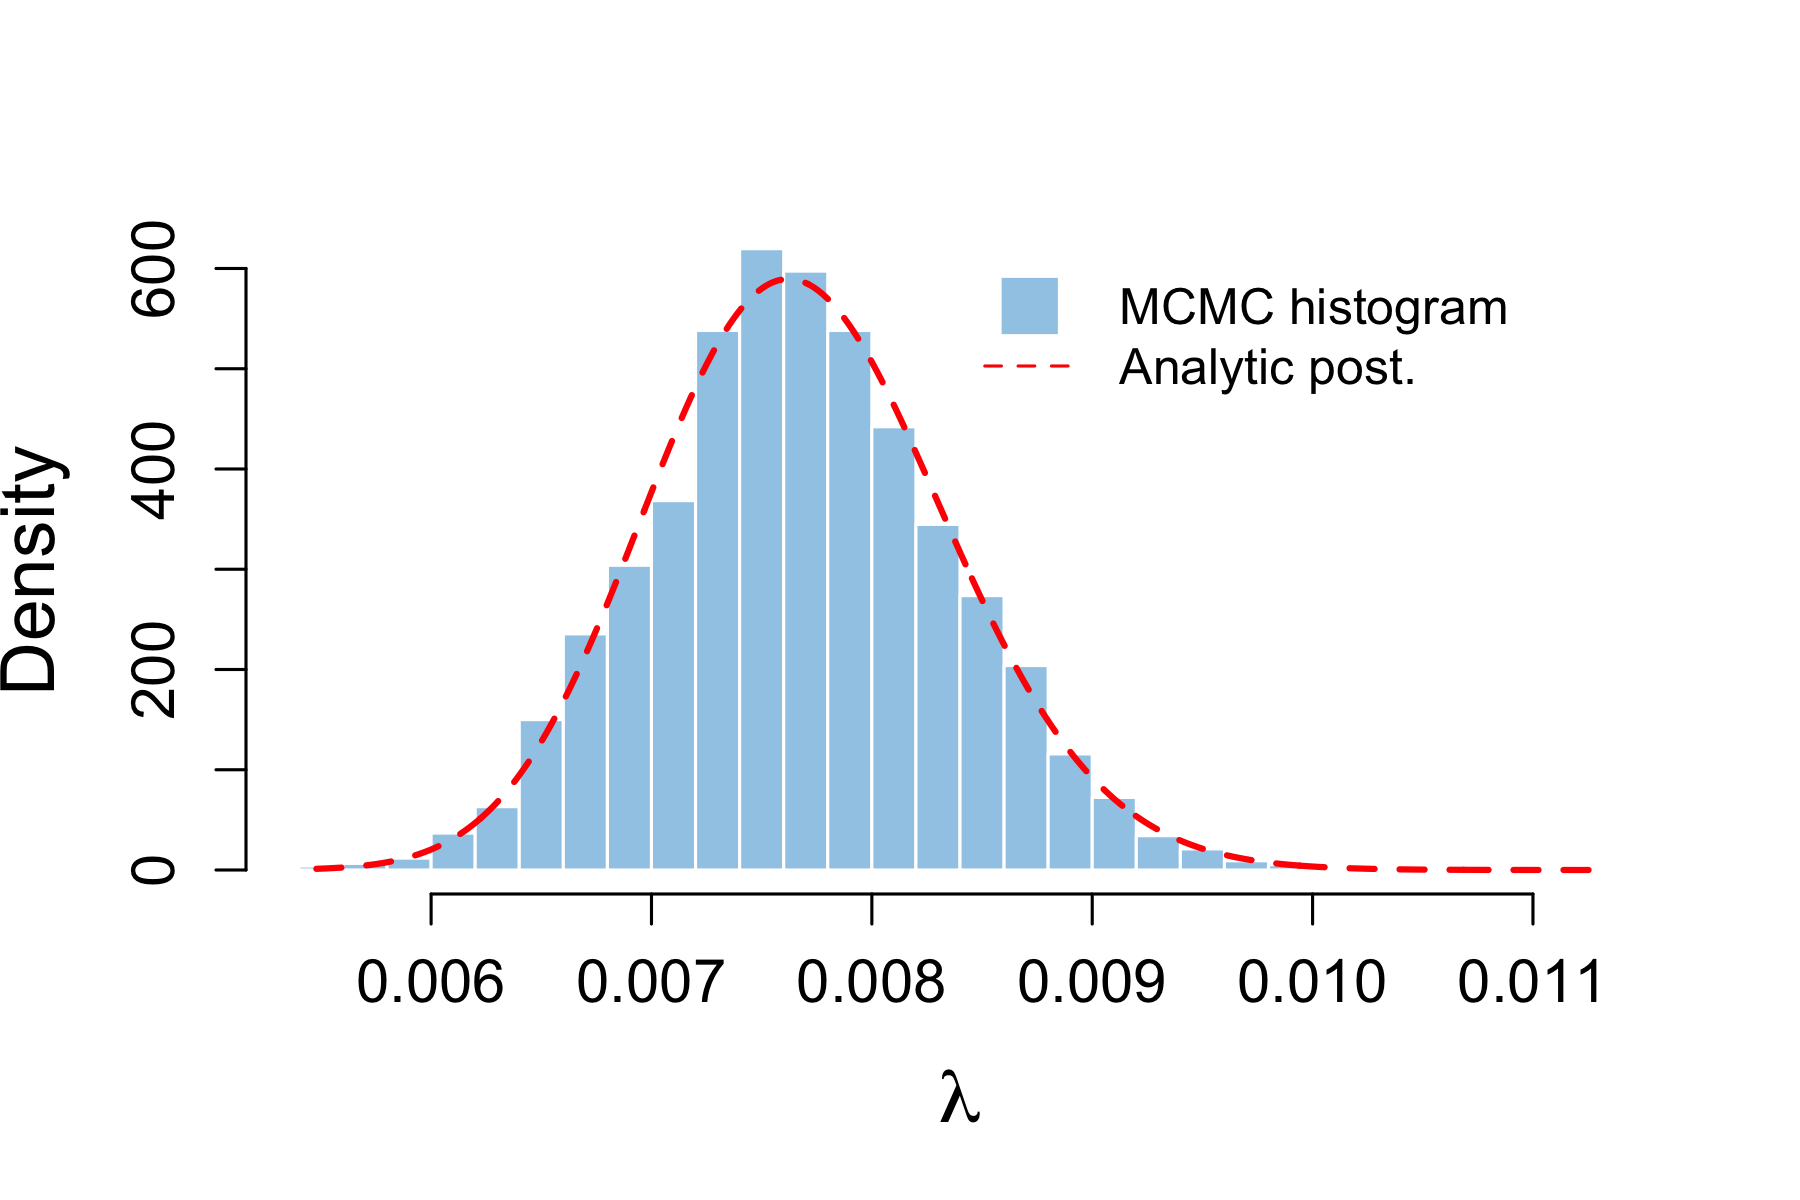
\includegraphics[height=8cm, width=0.5\textwidth]{images/veteran_post_lam.png}
    \caption{Posterior distribution of $\lambda$ from MCMC samples (histogram) and analytic Gamma posterior (red curve)}
    \label{fig:exp veteran}
\end{figure}


%%%%%%%%%%%%%%%%%%%%%%%%%%%%%%%%
%%%%%%%%%%%%%%%%%%%%%%%%%%%%%
%%%%这后面说的是后验预测
After obtaining the posterior distribution of model parameters $p(\theta \mid D)$, we are often interested in making predictions about future observations. This leads naturally to the posterior predictive distribution, defined as
\begin{equation}
    p(\tilde{y} \mid D) = \int p(\tilde{y} \mid \theta)\, p(\theta \mid D)\, d\theta
    \label{eq:18}
\end{equation}
where $\tilde{y}$ is a new (unseen) observation, $\theta$ denotes the model parameters, and $D$ is the observed dataset. In practice, this integral is often intractable and is therefore approximated using Monte Carlo methods. Specifically, we draw samples $\theta^{(1)}, \theta^{(2)}, \dots, \theta^{(M)}$ from the posterior $p(\theta \mid D)$, and estimate the posterior predictive distribution as
\begin{equation}
p(\tilde{y} \mid D) \approx \frac{1}{M} \sum_{m=1}^{M} p(\tilde{y} \mid \theta^{(m)}).
\end{equation}

\subsection{Model Checking}\label{sec:model checking}
\begin{figure}[H]
\centering
\resizebox{0.52\linewidth}{!}{
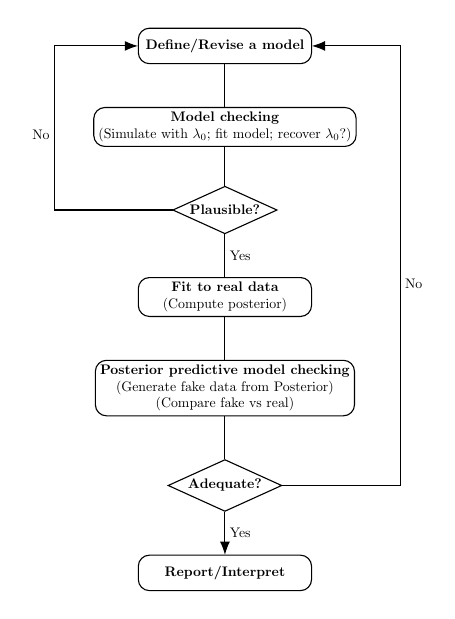
\begin{tikzpicture}[
 scale=0.50,
  every node/.style={transform shape}, 
  node distance=11mm,
  box/.style      ={rectangle, draw, rounded corners, align=center,
                    minimum width=44mm, minimum height=9mm},
  decision/.style ={diamond, aspect=2.2, draw, align=center, inner sep=1.4pt},
  ->, >=Latex
]

%--- Main process node ------------------------------------------------------
\node[box]      (model)   {\textbf{Define/Revise a model}};

\node[box]      (checking1)  [below=of model] {\textbf{Model checking} \\
(Simulate with $\lambda_0$; fit model; recover $\lambda_0$?)};

\node[decision] (pass1)   [below=10mm of checking1] {\textbf{Plausible?}};

\node[box]      (fit)     [below=of pass1]  {\textbf{Fit to real data}\\
(Compute posterior)};

\node[box]      (gen)     [below=of fit]    {\textbf{Posterior predictive model checking}\\
(Generate fake data from Posterior)\\
(Compare fake vs real)};

\node[decision] (pass2)   [below=of gen] {\textbf{Adequate?}};

\node[box]     (report)  [below=of pass2] {\textbf{Report/Interpret}};

%--- 连线 ------------------------------------------------------------
\draw (model)   -- (checking1)
      (checking1)  -- (pass1)
      (pass1)   -- node[right]{Yes}(fit)
      (fit)     -- (gen)
      (gen) -- (pass2)
      (pass2) -- node[right]{Yes}(report);

%--- Loopback ------------------------------------
\draw[->] (pass1.west) -- ++(-30mm,0) |- (model.west) node[pos=0.23, left]{No};
%\draw[->] (pass1.west) to[out=180,in=180,looseness=1.3] node[left]{No} (model.west);
\draw[->] (pass2.east) -- ++ (30mm,0 )|- (model.east) node[pos=0.23,right]{No};
\end{tikzpicture}}
\caption{General Bayesian workflow}
\end{figure}

\begin{tcolorbox}[
  title  = Algorithm 1: Simulating a Fake Survival Dataset (e.g.Posterior predictive model checking),
   fonttitle  = \small, 
  colback = white,
  colframe=black]
\textbf{Input}\\
\quad$\bullet$ posterior samples $\{\lambda^{(s)}\}$ \hfill (obtained by fitting real data)\\
\quad$\bullet$ sample size $n$ \hfill (same size as the real data set)\\
\quad$\bullet$ start‑time range $[a,0]$ with $a<0$ \\[6pt]
\textbf{Algorithm}\par
\begin{enumerate}
  \item Choose a single $\lambda^\ast$ from posterior samples \hfill (e.g.\ posterior mean)
  \item For $i = 1,\dots,n$
        \begin{enumerate}
          \item[] \hspace*{-10pt}%
          \begin{minipage}[t]{\linewidth}
          \begin{enumerate}
            \item Draw latent duration: $y_i \sim \operatorname{Exp}(\lambda^\ast)$
            \item Draw start time: $T_i \sim \operatorname{Uniform}(a,0)$
            \item Compute leaving time: $t_i = T_i + y_i$
            \item Observed pair $(\text{time}_i,\text{event}_i)$ \[\begin{aligned}
\text{if } \quad t_i &< 0: &&&\text{(event occurred before now)}\\
  &&\quad  \text{event}_i=1, &&\text{(uncensored)}\\ 
  &&\quad \text{time}_i=y_i
   &\quad \\
&\text{else}: &&&\text{(event in the future)}\\
   &&\quad \text{event}_i=0, &&\text{(right censored)}\\ 
   &&\quad \text{time}_i=-T_i &&\text{(time already spent)}
   &\quad 
\end{aligned}\]
          \end{enumerate}
          \end{minipage}
        \end{enumerate}
  \item Combine $(\text{time}_i,\text{event}_i)$ into a fake data set of size $n$.
\end{enumerate}
\label{fake data}
\end{tcolorbox}

\subsubsection{Model Checking via ECDF under Independent Censoring}
In model checking, to compare the overall distributional shapes of the real data and the simulated data, we use the empirical cumulative distribution function (ECDF) rather than histograms. Unlike histograms, ECDFs do not depend on subjective choices of bin widths and break points, thereby avoiding visual biases. Moreover, an ECDF is a monotone right-continuous step function defined on $[0,\infty)$, which stably displays differences between samples over the entire time axis. Importantly, ECDFs can be plugged directly into distance statistics such as the Kolmogorov–Smirnov or Cramér–von Mises metrics, facilitating quantitative assessment of model fit.

In survival data, the observed duration is determined jointly by the latent event time $T\ge 0$ and the censoring time $C\ge 0$. The observed quantity is
$$
Y=\min(T,C),\qquad \delta=\mathbf 1\{T\le C\}.
$$
That is, we observe the event time only when it is uncensored; otherwise, we observe the censoring time. Consequently, we split the data into two subsamples—an “event subsample’’ with $\delta=1$ and a “censored subsample’’ with $\delta=0$—and compute ECDFs for each subsample separately.

Under independent (non-informative) censoring, i.e., $T\perp C$, the two subsamples may be viewed as arising from two conditional distributions
\begin{itemize}
    \item for the event subsample ($\delta=1$), the observed values $Y=T$ follow the conditional distribution $T\mid(T\le C)$;
    \item for the censored subsample ($\delta=0$), the observed values $Y=C$ follow the conditional distribution $C\mid(C<T)$.
\end{itemize}
Let the event-subsample size be $n_1=\sum_i \delta_i$ and the censored-subsample size be $n_0=\sum_i (1-\delta_i)$. The corresponding empirical distribution functions are
\begin{equation}
    \widehat H_{\text{event}}(t)
=\frac{1}{n_1}\sum_{i:\,\delta_i=1}\mathbf 1\{Y_i\le t\},\qquad
\widehat H_{\text{cens}}(t)
=\frac{1}{n_0}\sum_{i:\,\delta_i=0}\mathbf 1\{Y_i\le t\},\qquad t\ge 0.
\end{equation}
By the Glivenko–Cantelli theorem (\cite{tucker1959generalization}), as sample sizes grow, these ECDFs converge uniformly to their respective target distribution functions
\begin{align}
\widehat H_{\text{event}}(t) &\xrightarrow{\text{uniformly in } t} H_{\text{event}}(t) := \Pr(T \le t \mid T \le C) \\
\widehat H_{\text{cens}}(t) &\xrightarrow{\text{uniformly in } t} H_{\text{cens}}(t) := \Pr(C \le t \mid C < T)
\end{align}
In summary, by splitting the data into event and censored subsamples and plotting their empirical distribution functions $\widehat H_{\text{event}}$ and $\widehat H_{\text{cens}}$, we can evaluate model fit within a unified framework along both dimensions.



%%%%%%%%%%%%%%%%%%%%%%%%%%%%%%%%%%%%%%%%%%%%%%%
\subsubsection{Choosing and Interpreting the Survey-Length Parameter $A$}

In the posterior predictive model checking of this study, we generate simulated data from the model and compare it with the observed data. This simulation relies on sampling given known quantities; a key quantity is the \textbf{maximum survey duration $A$ }in Algorithm 1 (\ref{fake data}), which is controlled by the user-specified parameter $a$, with the reparameterization $A = -a$, governing the censoring mechanism in the simulated data. In other words, $A$ sets the observation window in simulation and thereby affects both the censoring rate and the distribution of event times.

This quantity is not a parameter to be estimated by the model; it is an external input required to generate fake data. Although it may appear auxiliary, it is tightly coupled with model checking—different choices of $A$ change the censoring structure of the simulated data and therefore influence the credibility of posterior predictive results.

Does the observed data carry information about $A$? Yes. In any survival dataset, the “shadow” of the survey window is reflected in the censoring proportion and the shape of the observed durations. If the survey is short (small $A$), many subjects are censored before the event occurs, leading to a high right-censoring rate and “compressed” event times. Conversely, with a long survey (large $A$), more events are observed, censoring decreases, and event times spread out.

This can be seen in Figure~\ref{fig:离职数据分开的直方图} (histograms of event and censored durations in the employee turnover data). The number of events and censors is roughly balanced, suggesting that the survey was long enough to capture about half of the departures. Since the maximum observed duration exceeds 170 months, it is reasonable to infer that the underlying survey duration $A$ should be at least greater than 170; this directly informs how the censoring mechanism should be set in simulation.
\begin{figure}[H]
    \centering
    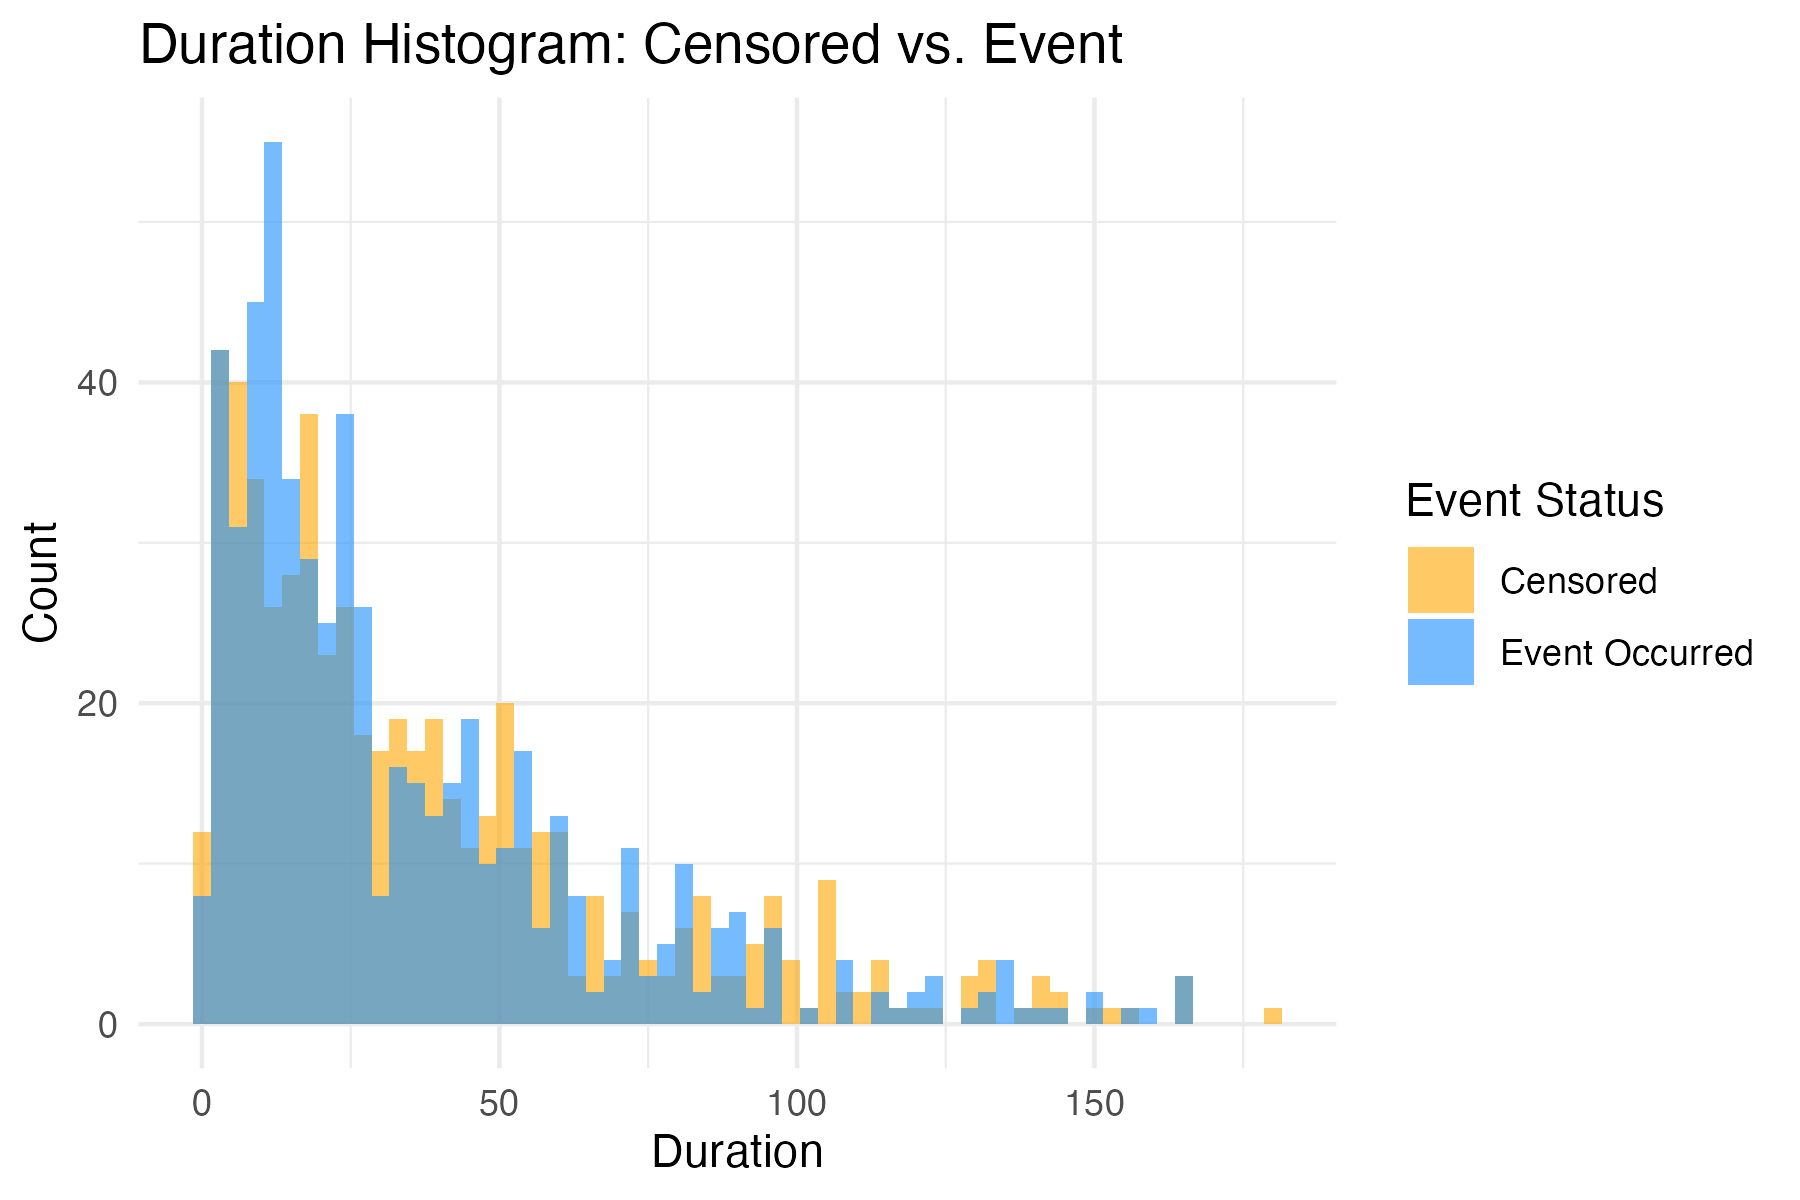
\includegraphics[height=5.5cm, width=0.6\textwidth]{images/separate_hist.png}
    \caption{Histograms of censored and event durations in the employee turnover data}
    \label{fig:离职数据分开的直方图}
\end{figure}
To further support this point, we simulate under two settings, $A = 30$ and $A = 1000$, and plot the empirical cumulative distribution functions (ECDFs) for both the event subsample ($\delta = 1$) and the censored subsample ($\delta = 0$), along with the histograms of simulated durations.
\begin{itemize}
    \item $A = 30$ (Figure~\ref{fig:ppc-A30}). Compared to the real-data histogram (Figure~\ref{fig:离职数据分开的直方图}), the simulated durations in Figure~\ref{fig:fake-hist_a30} are heavily compressed within 0–30 months, indicating that both events and censorings occur unusually early. Correspondingly, the ECDFs for events and censorings (Figure~\ref{fig:ecdf-cens_a30}~\ref{fig:ecdf-event_a30}, red lines) rise too steeply at short durations, deviating noticeably from the observed curves. This mismatch is primarily driven by an unrealistic observation window $A$, rather than a misfit of the event-time distribution (e.g., the parameter $\lambda$) itself.
    \item $A = 1000$ (Figure~\ref{fig:ppc-A1000})
  In contrast, Figure~\ref{fig:fake-hist_a1000} shows a histogram with a much wider and sparser spread of durations, and the ECDF curves (Figure~\ref{fig:ecdf-event_a1000}~\ref{fig:ecdf-cens_a1000}, red lines) align more closely with the observed data. However, when compared to the real-data histogram in Figure~\ref{fig:离职数据分开的直方图}, this setting exceeds any realistic survey length—implying a maximum tenure close to 83 years—which is implausible in practical employment contexts. Thus, although the simulated curves fit better visually, this apparent “match” relies on an unrealistic assumption about $A$, and should not be accepted as a reliable model-checking result.
\end{itemize}
These two examples reinforce a key point: when performing posterior predictive checks, fit quality must be evaluated alongside the realism of the data-generating assumptions in simulation.
\begin{figure}[htbp]
\centering
\begin{subfigure}[t]{0.3\textwidth}
  \centering
  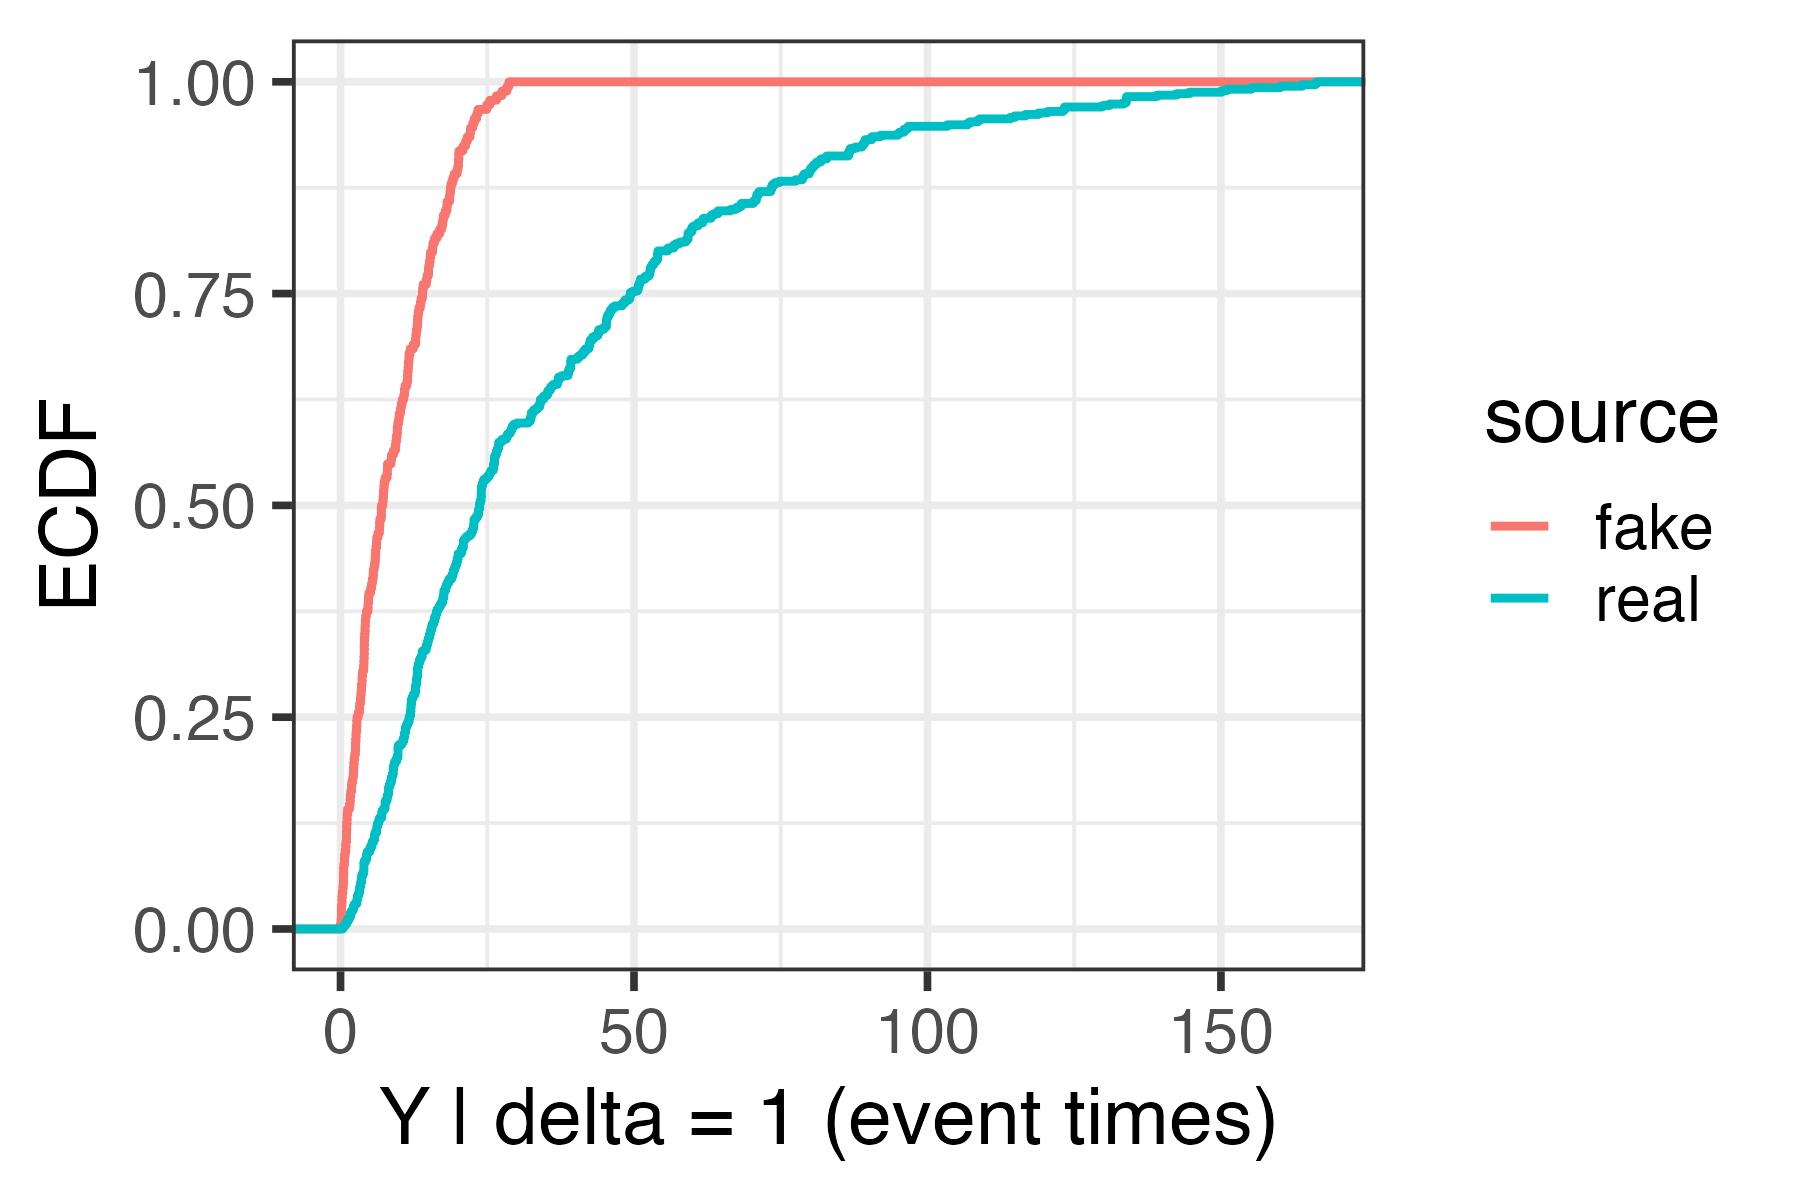
\includegraphics[width=\linewidth]{images/ppc_event_ecdf_A30.png}  % 图1路径
  \caption{ECDF of $Y \mid \delta=1$}
  \label{fig:ecdf-event_a30}
\end{subfigure}\hfill
\begin{subfigure}[t]{0.3\textwidth}
  \centering
  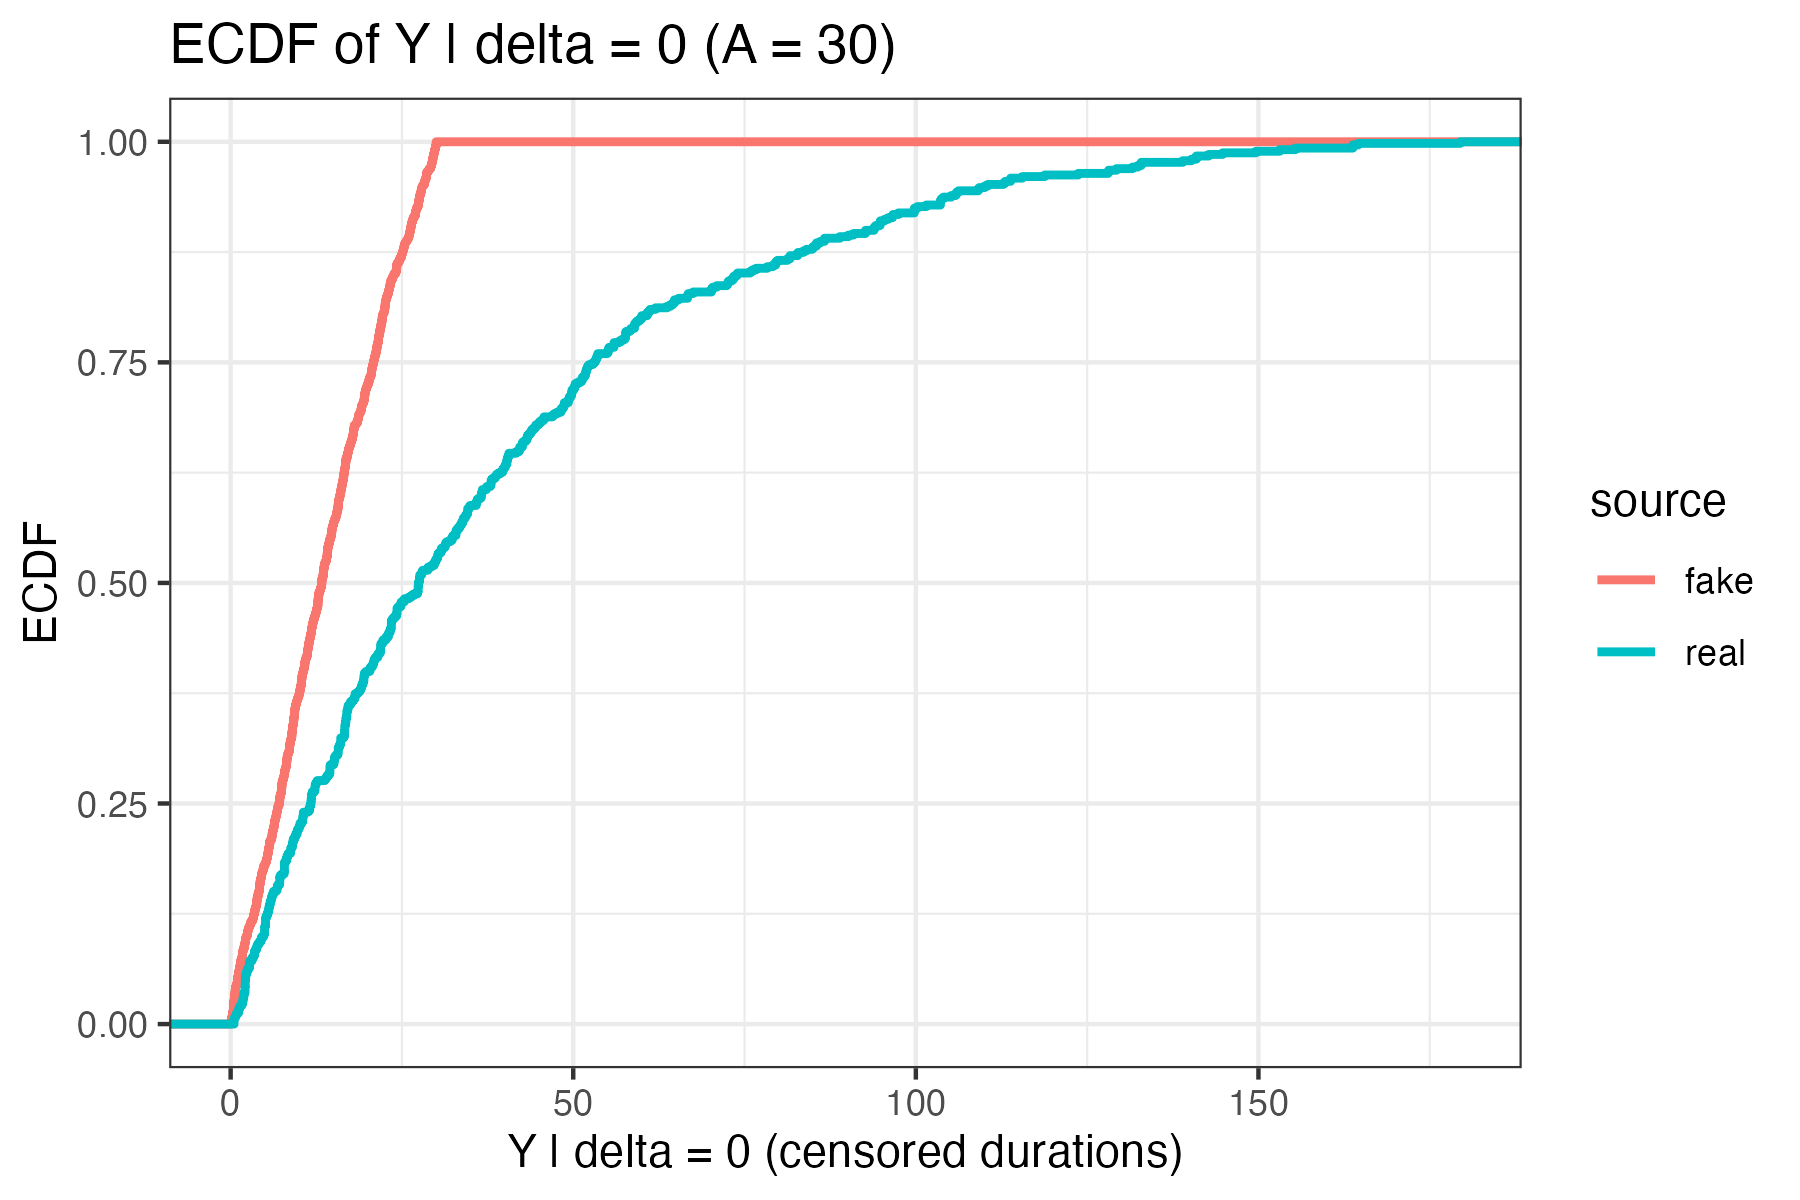
\includegraphics[width=\linewidth]{images/ppc_censored_ecdf_A30.png}   
  \caption{ECDF of $Y \mid \delta=0$}
  \label{fig:ecdf-cens_a30}
\end{subfigure}\hfill
\begin{subfigure}[t]{0.37\textwidth}
  \centering
  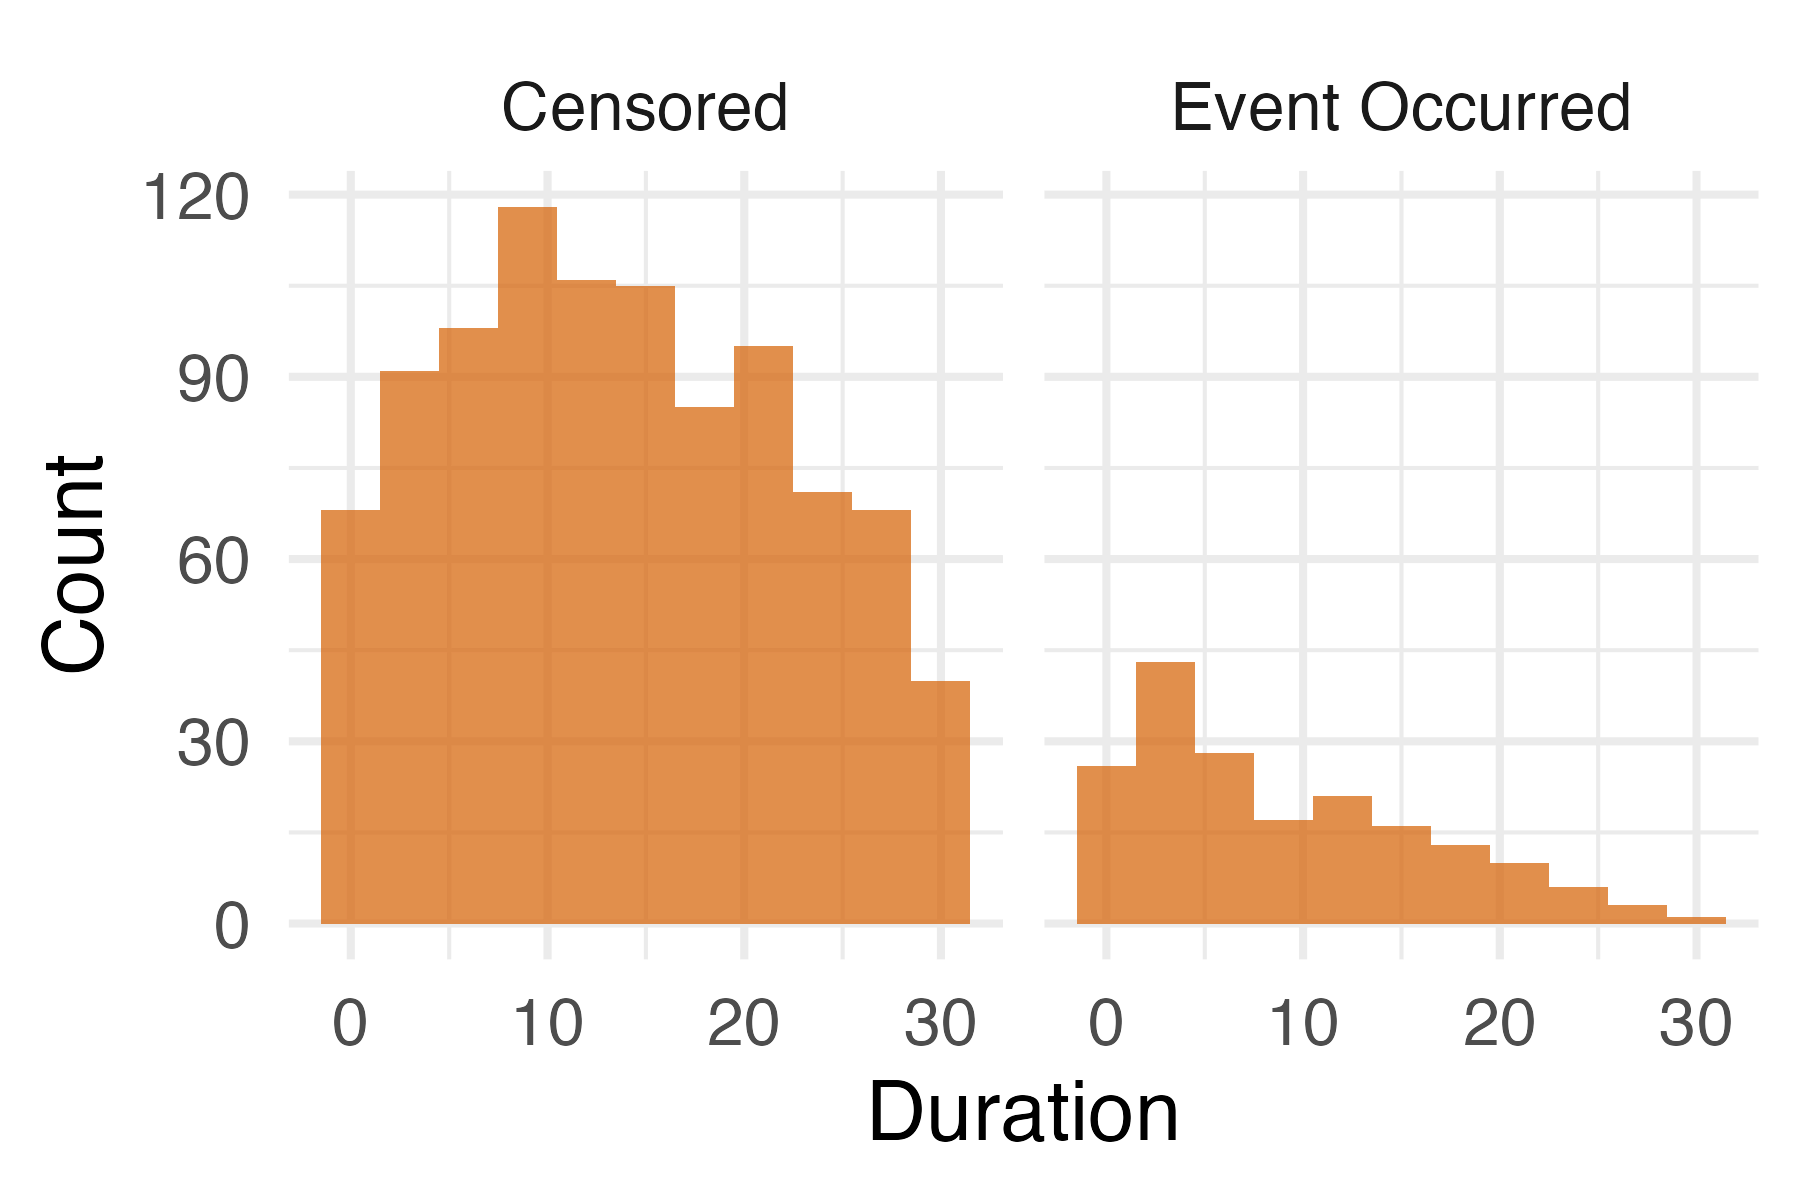
\includegraphics[width=\linewidth]{images/fake_duration_hist_a30.png}   % 图3路径
  \caption{Fake-data histogram}
  \label{fig:fake-hist_a30}
\end{subfigure}
\caption{Posterior predictive checking ($A=30$).}
\label{fig:ppc-A30}
\end{figure}
%%%%%%%%%%%%%%%%%%%%%%
\begin{figure}[htbp]
\centering
\begin{subfigure}[t]{0.3\textwidth}
  \centering
  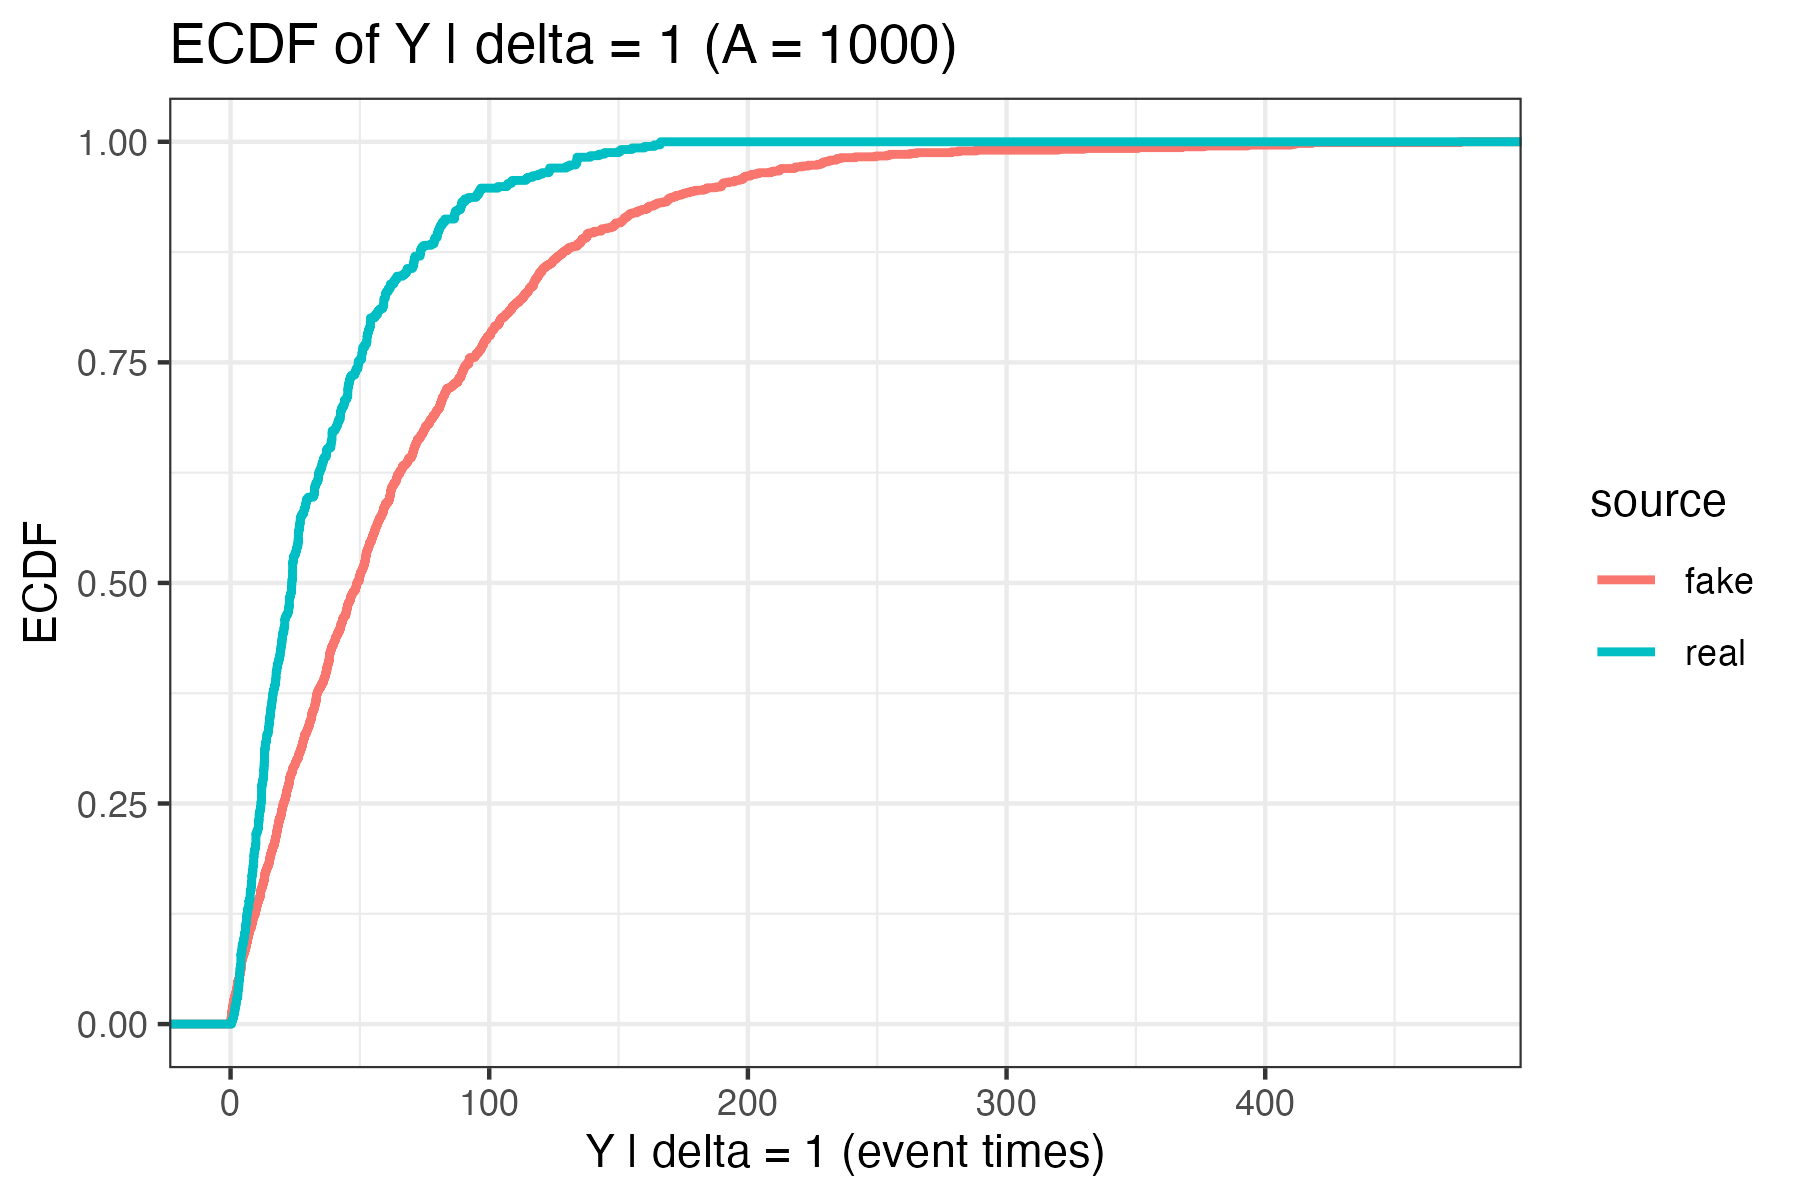
\includegraphics[width=\linewidth]{images/ppc_event_ecdf_A1000.png}  % 图1路径
  \caption{ECDF of $Y \mid \delta=1$}
  \label{fig:ecdf-event_a1000}
\end{subfigure}\hfill
\begin{subfigure}[t]{0.3\textwidth}
  \centering
  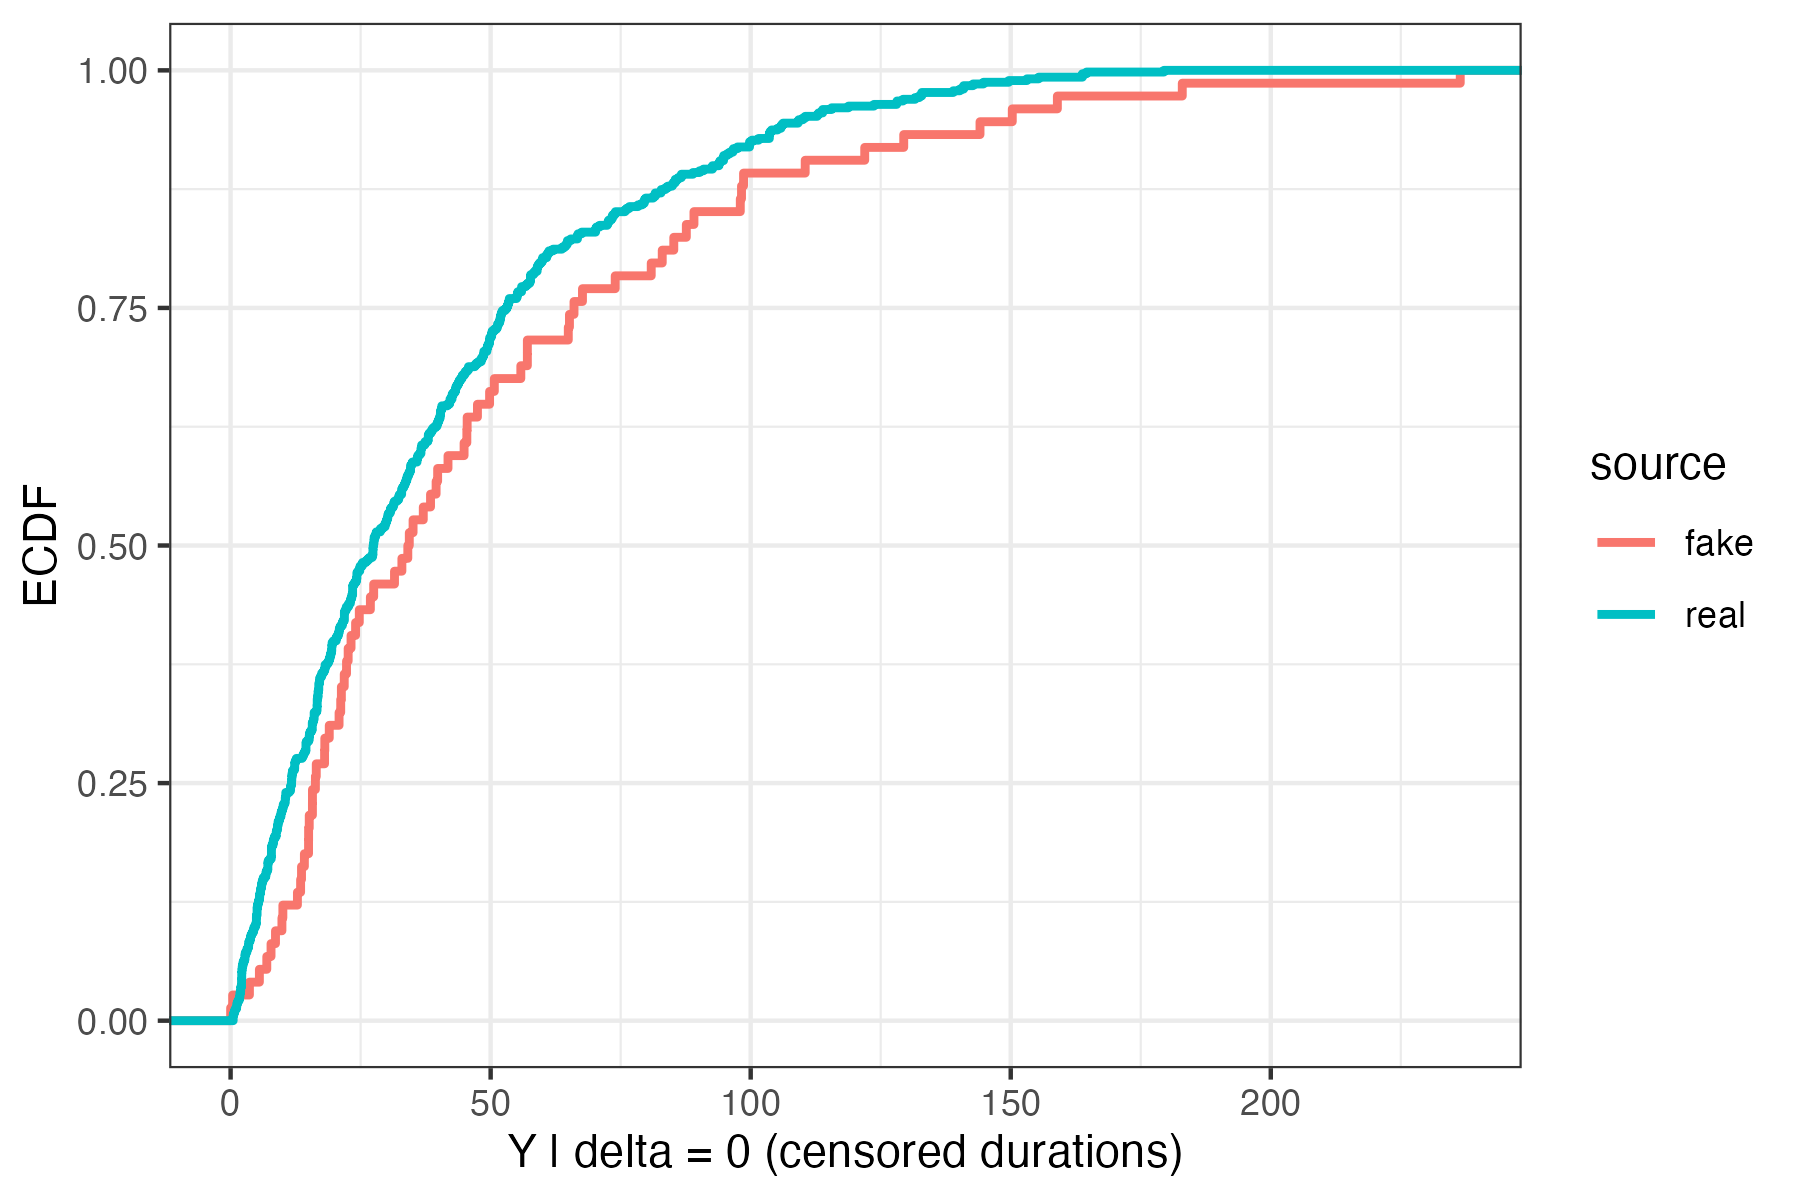
\includegraphics[width=\linewidth]{images/ppc_censored_ecdf_A1000.png} 
  \caption{ECDF of $Y \mid \delta=0$}
  \label{fig:ecdf-cens_a1000}
\end{subfigure}\hfill
\begin{subfigure}[t]{0.37\textwidth}
  \centering
  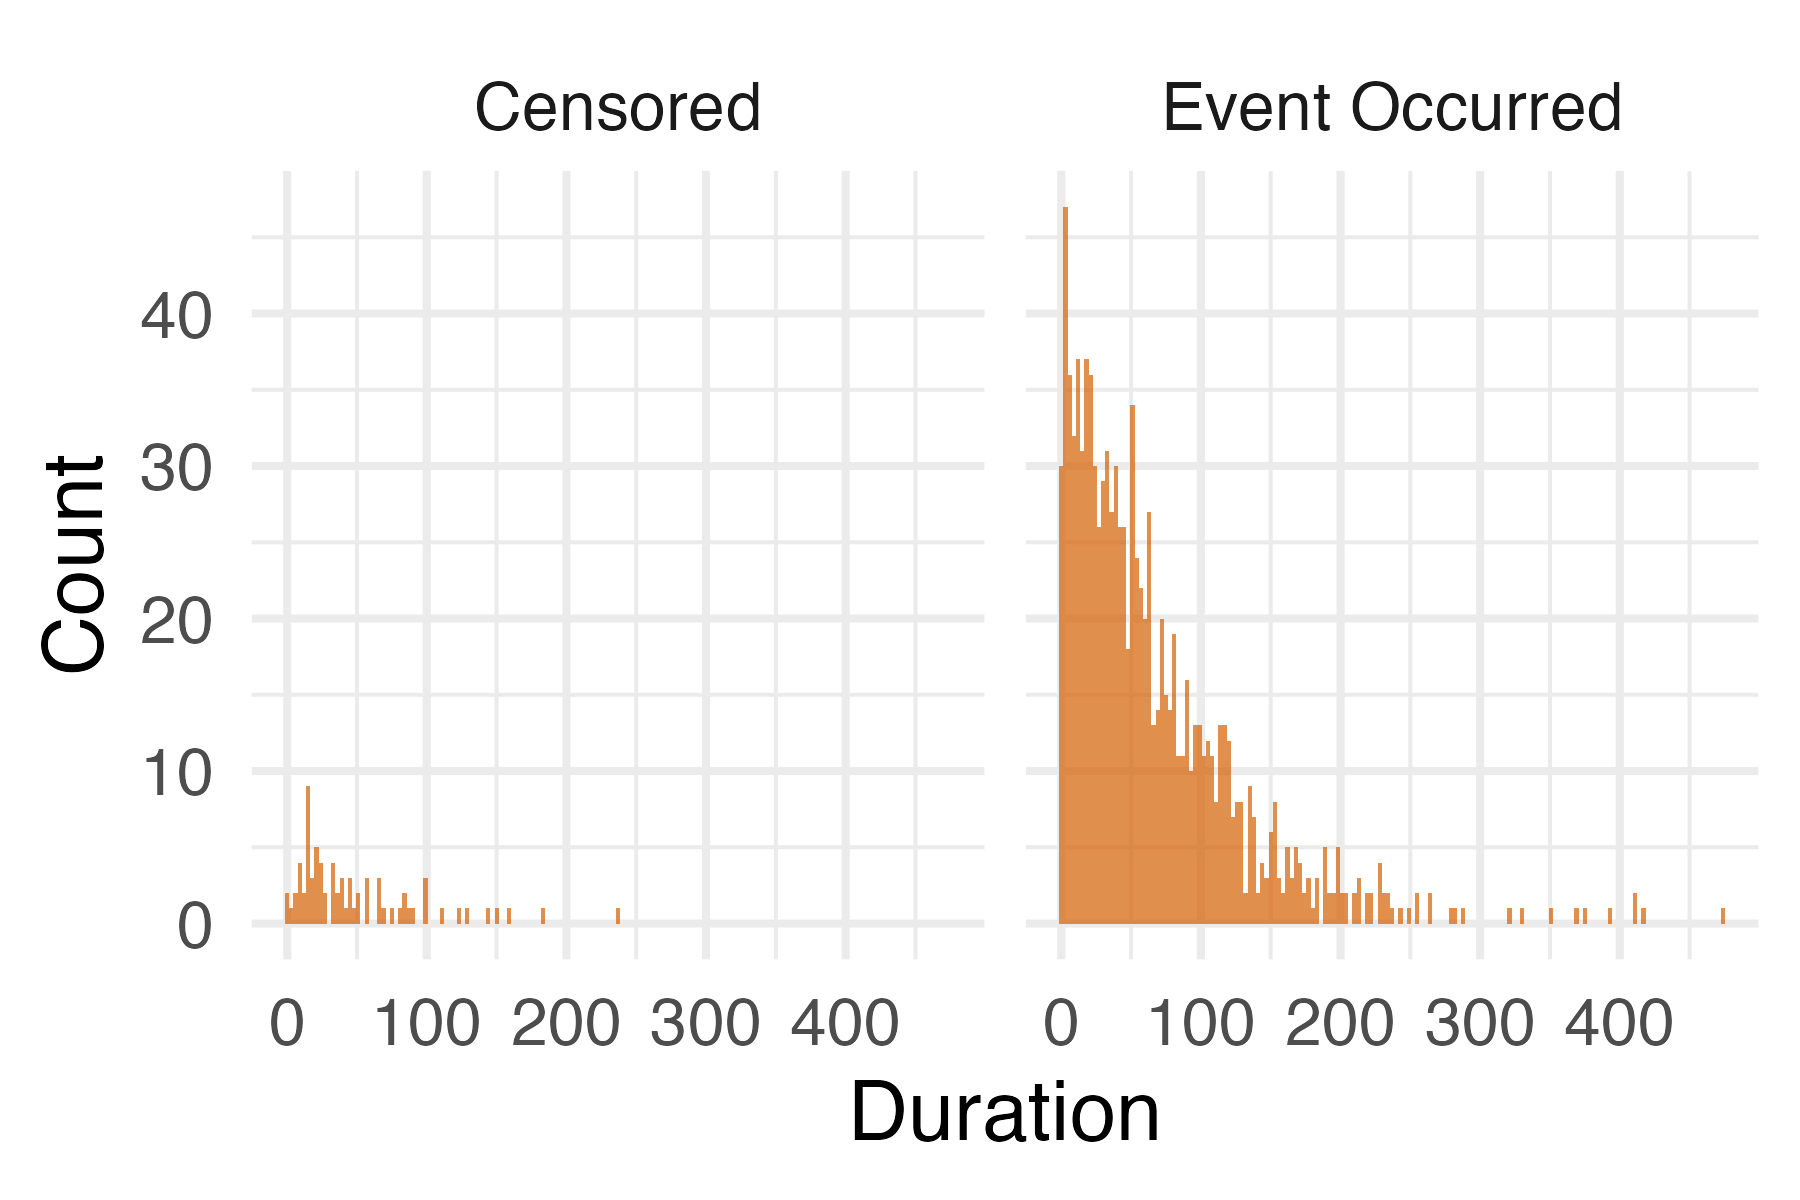
\includegraphics[width=\linewidth]{images/fake_duration_hist_a1000.png}   % 图3路径
  \caption{Fake-data histogram}
  \label{fig:fake-hist_a1000}
\end{subfigure}
\caption{Posterior predictive checking ($A=1000$).}
\label{fig:ppc-A1000}
\end{figure}


%\subsection{Posterior predictive CDF}
%\input{MSc_Statistics_Research_Report_paper/section/Methods_subsection/posterior predictive cdf }


























\section{Results}
\subsection{Posterior Inference under the Extended Model}
\label{res:post_contour}
Figure~\ref{fig:contour} displays the joint posterior distribution of $(\lambda, A)$, together with the MAP estimate and the corresponding HPD regions. The posterior mode is located at $\lambda \approx 0.0138$ and $A = y_{\max} \approx 179.45$ months, indicating that the estimate of $A$ coincides exactly with the longest observed tenure in the data. This suggests that the posterior inference of $A$ is strongly driven by the boundary constraint rather than by additional evidence from the data.

First, the posterior distribution of $\lambda$ is highly concentrated, with a relatively narrow range. This shows that the event rate parameter $\lambda$ is primarily determined by the observed event times and can therefore be estimated with high precision. By contrast, the uncertainty associated with $A$ is substantially larger.

Second, the HPD regions exhibit a clear truncation effect at the boundary $A = y_{\max}$. Since the model enforces $A \geq y_{\max}$, the posterior mass is forced against this boundary, creating a sharp cutoff on the left. As a result, the MAP point falls exactly on the boundary, while the 86.5\% HPD region extends almost entirely upward along this edge, forming a one-sided expansion rather than a symmetric spread around the mode, as would be typical under a Gaussian distribution. In other words, the uncertainty in $A$ is essentially about “how much larger than $y_{\max}$ it could be,” rather than about symmetric fluctuations around the MAP.

A closer comparison of the HPD regions further reinforces this interpretation: if the posterior were approximately Gaussian and independent, the 39.3\% and 86.5\% regions would resemble concentric ellipses. In contrast, here the outer region expands asymmetrically in the $A$ direction and clings to the boundary, revealing a boundary-driven skewness rather than Gaussian-like symmetric tails. The slight tilt of the contour also suggests a weak dependence between $\lambda$ and $A$, reflecting the fact that the censoring window and event rate jointly shape the observed data. However, this dependence is secondary compared with the strong boundary effect dominating the inference for $A$.

This observation naturally motivates the marginalization analysis in the next section. By integrating out $A$, we can check whether the extended formulation remains consistent with the baseline exponential model in terms of $\lambda$, thereby clarifying to what extent the introduction of $A$ truly alters—or preserves—the original inferential structure.
\begin{figure}[H]
    \centering
    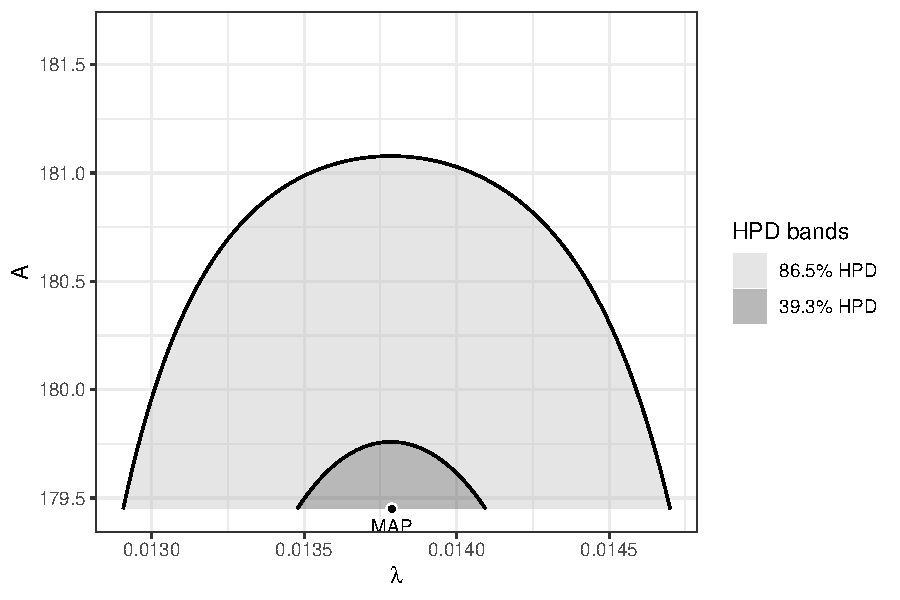
\includegraphics[height=9cm, width=0.65\textwidth]{images/post_contour.pdf}
    \caption{{\small Joint posterior $p(\lambda,A\mid\mathcal D)$ with 39.3\%/86.5\% HPD contours and MAP (black).}}
    \label{fig:contour}
\end{figure}


\subsection{Marginalization and Consistency Check}
\label{res:marginal}
Building on the boundary-driven geometry in Section~\ref{res:post_contour}, we now ask whether introducing $A$ changes inference on $\lambda$ once we focus on $\lambda$ alone. Figure~\ref{fig:marginal} compares the marginal posterior of $\lambda$ obtained from the extended model (blue; integrating out $A$ on the grid) with the analytic posterior from the baseline exponential model that does not include $A$ (red).

The two curves are visually indistinguishable across the entire support: the peak location, peak height, and tail decay coincide to plotting precision, and the associated credible intervals match to numerical accuracy. This confirms a key point for practice: Inference on $\lambda$ is preserved after introducing $A$. In the extended model, $A$ behaves as a (predictive) nuisance parameter: it is crucial for generating realistic fake data and for describing the observation window, but it does not alter the posterior for the event-time rate $\lambda$.

This empirical agreement is exactly what the factorization of the likelihood predicts (see Section~\ref{边际化章节}): the $\lambda$-dependent and $A$-dependent terms separate, so integrating over $A$ contributes only a normalizing constant that does not depend on $\lambda$. Consequently, the boundary-driven skewness seen along the $A$ direction in Section~\ref{res:post_contour} does not propagate into the marginal for $\lambda$.

\begin{figure}[H]
    \centering
    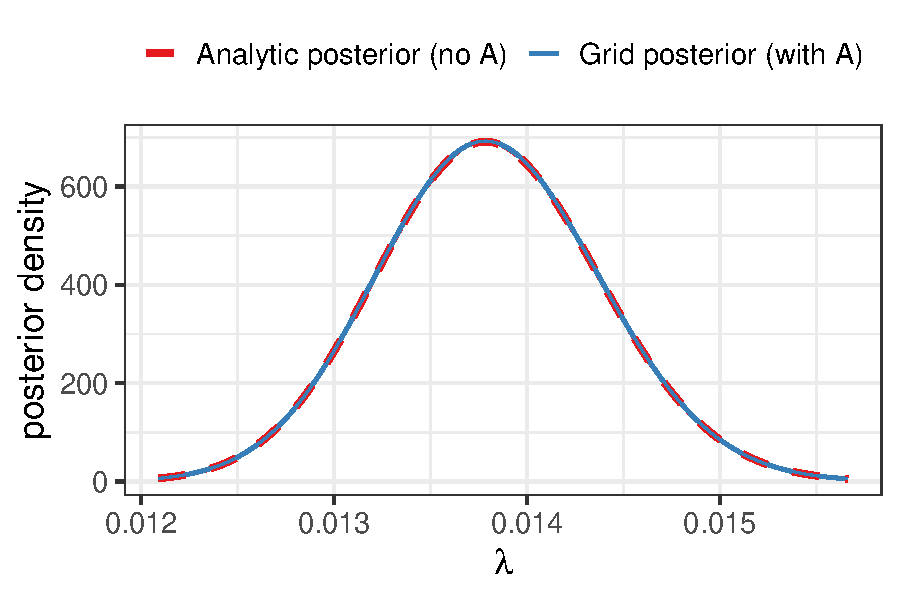
\includegraphics[height=6cm, width=0.7\textwidth]{images/lambda_marginal_compare.pdf}
    \caption{{\small Marginal posterior of $\lambda$ under the extended model (blue, obtained by integrating out $A$) versus the analytic posterior under the baseline exponential model (red).}}
    \label{fig:marginal}
\end{figure}
To further examine the stability of the marginal posterior for $\lambda$, we compared two sharply different priors for $A$: a weakly informative uniform prior $[y_{\max}, y_{\max}+500]$ and a truncated normal prior centered around $y_{\max}+50$. As shown in Figure~\ref{fig:diff_A_marginal}, despite the substantial difference in prior shapes, the resulting marginal posteriors for $\lambda$ are virtually identical.

This robustness is fully consistent with the theoretical result in equation~\eqref{eq:47} in Section~\ref{边际化章节}. As long as the prior for $A$ is independent of $\lambda$, integrating out $A$ contributes only a constant factor. Consequently, the marginal posterior of $\lambda$ is determined entirely by its likelihood and remains unaffected by the specific form of the prior on $A$.
\begin{figure}[H]
    \centering
    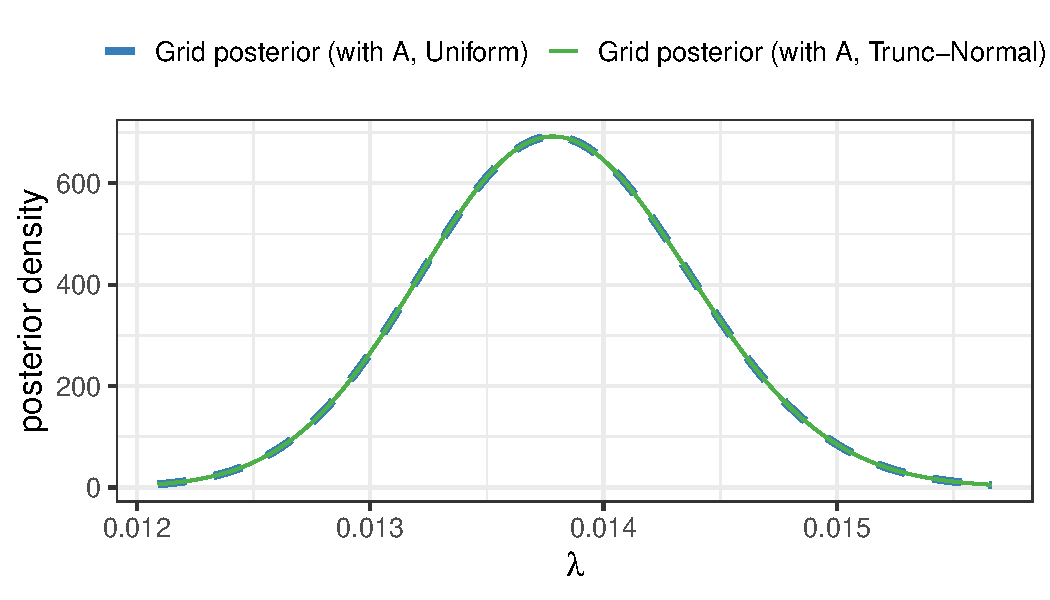
\includegraphics[height=6cm, width=0.75\textwidth]{images/diff_A_prior_marginal_compare.pdf}
    \caption{{\small Marginal posterior of $\lambda$ under two priors for $A$: uniform $[y_{\max}, y_{\max}+500]$ (blue) and truncated normal near $y_{\max}+50$ (green).}}
    \label{fig:diff_A_marginal}
\end{figure}

\subsection{Baseline Model Fit and Limitations}
\label{res:baseline_ecdf}
While Section~\ref{res:marginal} showed that marginalizing out $A$ preserves the baseline inference on $\lambda$, such consistency does not guarantee that the baseline model itself adequately reflects the data. To further assess its validity, we first perform a simulation-based model check. Specifically, we generated pseudo-data with a fixed value $\lambda=0.05$ and refitted the exponential model. As shown in Table~\ref{tab:post-ci}, the posterior mean (0.053) and 95\% CrI [0.0496, 0.0567] successfully recover the true value, indicating that the model is structurally sound. For completeness, the full posterior histogram is provided in Supplementary Figure~\ref{fig:posterior_s1}.
\begin{table}[H]
\centering
\caption{{\small Posterior summaries and 95\% credible intervals (simulation-based model check)}}
\label{tab:post-ci}
\small
\begin{tabular}{lccccc}
\toprule
{Parameter} & {Mean} & {2.5\%} & {97.5\%} & {$n_{\text{eff}}$} & {Rhat} \\
\midrule
$\lambda$   & 0.0531 & 0.0496 & 0.0567 & 1113 & 1.000 \\
\bottomrule
\end{tabular}
\end{table}
Having established that the baseline model is structurally coherent, we next examine its adequacy when applied to real data. In the posterior predictive model checking of the baseline specification, the true value of the observation-window parameter $A$ is unknown. Section~\ref{Impact of A} illustrated the distributional consequences of three candidate values, $A=30, \,200,$ and $1000$ months. Here, we concentrate on the two extremes, $A=30$ and $A=1000$, to examine how the baseline model behaves under contrasting window lengths. Posterior predictive checks under these settings yield the empirical cumulative distribution functions (ECDFs) shown in Figures~\ref{fig:ppc_a30}~\ref{fig:ppc_a1000}, which are compared against the real data.

\textbf{Case $A=30$ (Figure~\ref{fig:ppc_a30}):} For both event times and censored durations, the predictive ECDFs rise sharply in the early period and deviate strongly from the observed curves. The simulated curves are nearly linear, approximating a uniform distribution, which implies that the model expects most individuals to either fail or be censored within a short window. This eliminates the exponential decay pattern visible in the real data. The corresponding counts are events = 184 and censored = 945 (Table~\ref{tab:modelcheck_counts}), which differ drastically from the real data (events = 571, censored = 558), with the censored proportion being far too high. The histograms (Figure~\ref{fig:fake-hist_a30} in Section~\ref{Impact of A}) likewise show that durations are artificially compressed into the 0–30 month range. This indicates that when $A$ is too small, the model mechanically forces most individuals into “premature censoring,” leading to a breakdown of the fit.

\textbf{Case $A=1000$ (Figure~\ref{fig:ppc_a1000}):} The predictive ECDFs appear superficially closer to the real curves, particularly in the tail, where the discrepancy is less obvious. However, the corresponding counts (events = 1055, censored = 74) are highly imbalanced, with almost all individuals predicted to experience the event. The histograms (Figure~\ref{fig:fake-hist_a1000}) confirm that durations are stretched into implausibly long tails. This explains why the ECDFs look deceptively close to the observed data: with almost no censored individuals, nearly all samples are forced onto the “event curve,” which smooths the overall shape. Yet this apparent fit is spurious, as it distorts the censoring mechanism and fails to capture the structural properties of the data.

\begin{table}[H]
\centering
\caption{{\small Event and censoring counts in real and simulated datasets (model checking)}}
\label{tab:modelcheck_counts}
\small  
\begin{tabular}{lcc}
\toprule
\textbf{Dataset} & \textbf{Censoring ($0$)} & \textbf{Events ($1$)} \\
\midrule
Real data        & 558  & 571  \\
Simulated ($A=30$)   & 945  & 184  \\
Simulated ($A=1000$) & 74   & 1055 \\
\bottomrule
\end{tabular}
\end{table}

\begin{figure}[H]
    \centering
    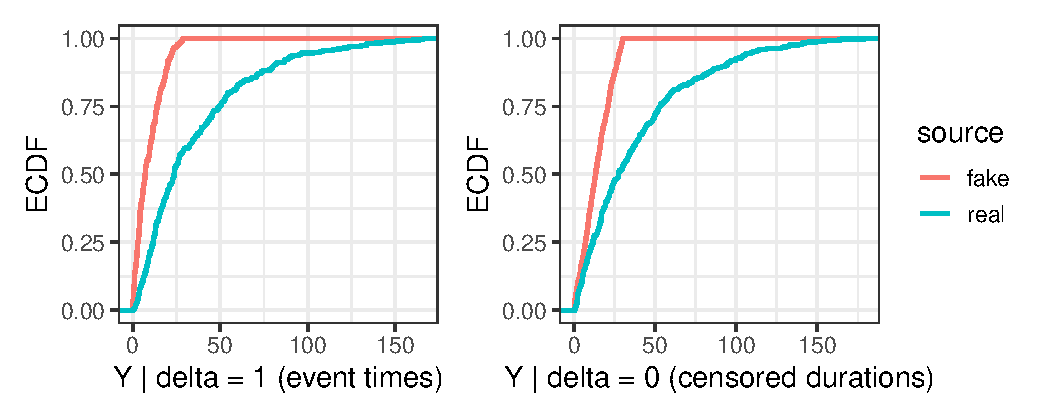
\includegraphics[height=4cm, width=0.8\textwidth]{images/ppc_two_a30.pdf}
    \caption{{\small Posterior predictive ECDFs of event times (left) and censored durations (right) under fixed $A=30$.}}
    \label{fig:ppc_a30}
\end{figure}

\begin{figure}[H]
    \centering
    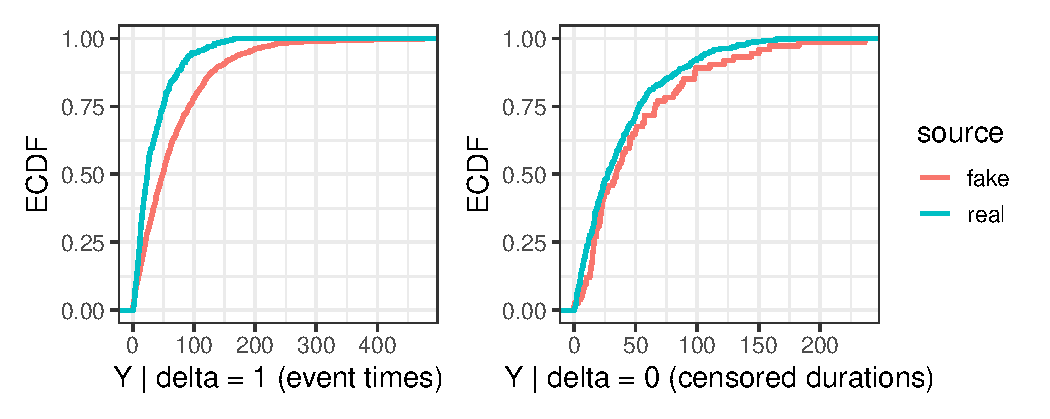
\includegraphics[height=4cm, width=0.8\textwidth]{images/ppc_two_a1000.pdf}
    \caption{{\small Posterior predictive ECDFs of event times (left) and censored durations (right) under fixed $A=1000$.}}
    \label{fig:ppc_a1000}
\end{figure}
These results highlight a structural mismatch: the baseline exponential model cannot reproduce the censoring pattern observed in the data. To address this, we turn to the extended model with the observation-window parameter $A$ and evaluate its performance through posterior predictive model checking.


\subsection{Posterior Predictive Model Checking (Extended Model)}

The baseline model failed to reproduce the censoring structure, underscoring the need for an extended specification. By introducing the observation-window parameter $A$, the model is able to capture this structural feature. The joint posterior yields MAP estimates of $\lambda \approx 0.0138$ and $A \approx 179$, which are consistent with the intuitive setting of $A \approx 200$ discussed in Section~\ref{Impact of A}. This consistency illustrates how the Bayesian framework can formalize and refine prior intuition.

Posterior predictive checks based on the MAP estimates demonstrate clear improvements in reproducing the observed data. For event times, the MAP-simulated ECDF (Figures~\ref{fig:ppc_map}) aligns closely with the empirical curve, especially in the early growth phase, indicating that the model captures the dynamics of event occurrence accurately. In contrast, the $A=1000$ specification produces a noticeably flatter curve, reflecting an underestimation of early event rates, even though its tail appears superficially smooth.

For censored durations, the MAP fit is again more reasonable. While some discrepancies remain, the distributional structure is much closer to the real data: censored observations are spread across the 0–180 month range with a smooth decline in frequency, as shown in the histogram~\ref{fig:fake_map}. This avoids the over-compression seen under $A=30$ as well as the near-elimination of censoring under $A=1000$, where apparent curve alignment arises only from proportional effects rather than a faithful representation of the censoring mechanism.

Overall, the MAP-based extended model not only reproduces the shape of the ECDFs but also recovers the structural balance between events and censoring. These results highlight the substantive improvement of the extended specification over the baseline model.
\begin{figure}[H]
    \centering
    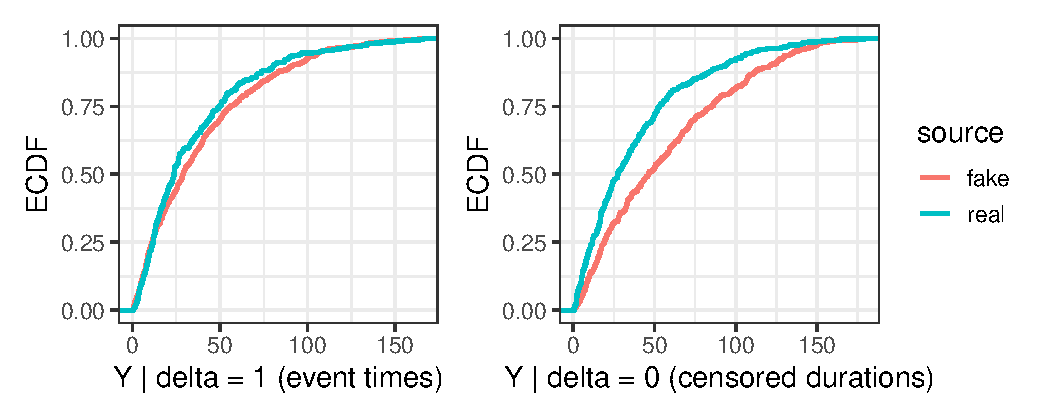
\includegraphics[height=4cm, width=0.8\textwidth]{images/ppc_two_map.pdf}
    \caption{{\small Posterior predictive ECDFs of event times (left) and censored durations (right) under the MAP estimates ($\lambda \approx 0.0138, A \approx 179$)}}
    \label{fig:ppc_map}
\end{figure}

\begin{figure}[H]
    \centering
    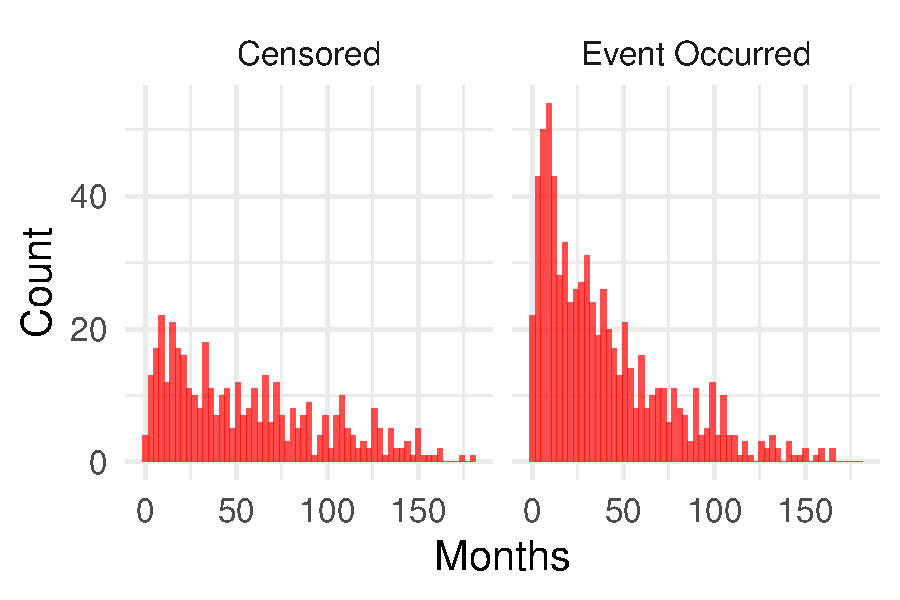
\includegraphics[height=5cm, width=0.6\textwidth]{images/fake_duration_hist_Apost.pdf}
    \caption{{\small Posterior predictive histograms of event times (right) and censored durations (left) under the MAP estimates ($\lambda \approx 0.0138, A \approx 179$)}}
    \label{fig:fake_map}
\end{figure}

\section{Discussion}
The preceding results examined various aspects of model fit, and Sections~\ref{res:post_contour} and~\ref{res:marginal} highlight an especially intriguing finding. Specifically, the marginal posterior of $\lambda$ is unaffected by the prior choice on $A$, as long as the support condition $A \geq y_{\max}$ is satisfied. This separability is unusual in multi-parameter Bayesian survival models, where parameters typically remain entangled and sensitive to prior assumptions. Here, however, the inference for the event-rate parameter $\lambda$ remains robust, while $A$ serves only to capture the structural features of the censoring mechanism. In practical terms, this means $\lambda$ can always be stably estimated, while $A$ captures censoring structure without distorting inference on the underlying hazard rate. 

While this theoretical robustness is reassuring, posterior predictive checks simultaneously reveal practical shortcomings of the exponential baseline. As shown in Section~\ref{res: model checking}, the constant hazard assumption fails to capture the empirical feature of the data, namely a “steep early rise followed by a gradual decline.” This results in a systematic underestimation of event occurrences in the mid-range. To address this mismatch, it is natural to consider alternative distributions, especially those that allow hazards to vary over time and possibly take non-monotonic forms.

Before moving to such flexible specifications, however, it is natural to first reflect on a monotone alternative: the Weibull model. Although Weibull introduces time dependence, its single shape parameter limits flexibility, making it difficult to accommodate both the sharp early risk and the smoother decline in later periods (as illustrated more clearly in the supplementary figures, such an adjustment does not lead to noticeable improvement). Hence, models with monotone hazards are not suitable for this dataset. This reflection points toward a more promising direction: models that allow non-monotone and locally curved baseline hazards.

A natural candidate is the piecewise-constant hazard (PWE) model. Dividing time into intervals permits the hazard to vary flexibly across segments, thereby directly capturing the “early steep, later flat” turnover pattern observed in the data. Here, I illustrate this approach with a simplified version using six segments, while keeping the observation window fixed at $A=179$ for comparability with the exponential model. The posterior predictive results show that the ECDF of event times improves markedly, indicating that such models align more closely with the structure of the data.
\begin{figure}[H]
    \centering
    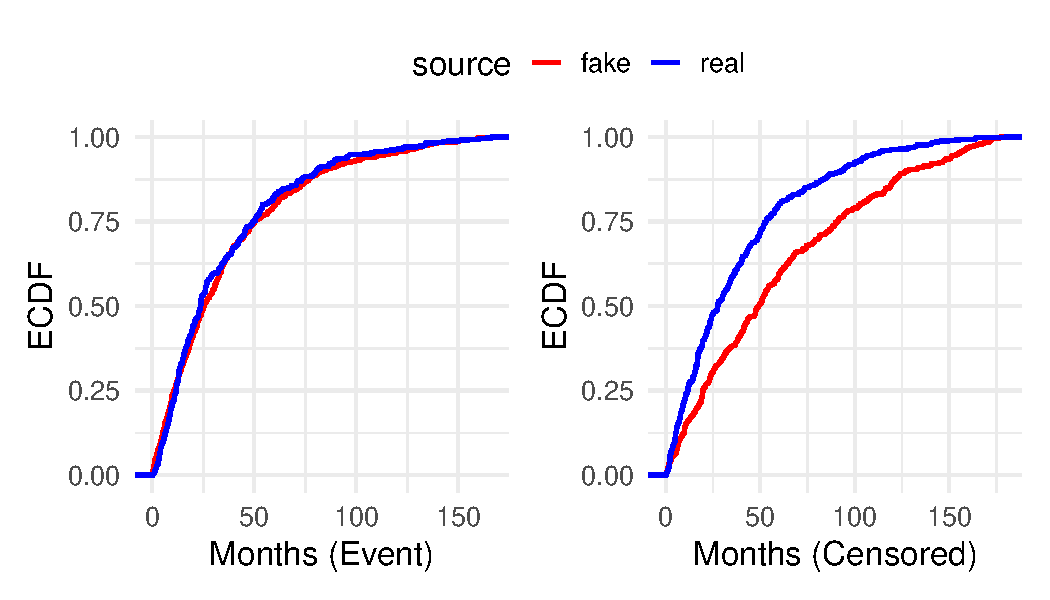
\includegraphics[height=6cm, width=0.75\textwidth]{images/piece6_ecdf_comparison.pdf}
    \caption{{\small Posterior predictive ECDFs of event times (left) and censored durations (right) under a six-segment piecewise-constant hazard model (cuts at 40, 75, 105, 120, 160, 200), with $A=179$ fixed for comparability.}}
    \label{fig:ppc_map}
\end{figure}
However, this exercise also reveals another issue that even under the PWE framework, the fit for censoring remains problematic. The observed censoring ECDF lies systematically above the simulated one. This discrepancy does not arise from the event process but rather from the censoring mechanism. In the current PPC setting, we assume uniform entry over $[0, A]$, such that censoring is entirely administrative. In reality, however, recruitment may not be uniform—for instance, if the company recruits heavily in later periods, this would generate more early censoring. This explains the “excess censoring” observed in the real data and suggests that future work should incorporate entry mechanisms informed by the company’s operational context.

Finally, it is important to note that modeling choices depend on research objectives. If the aim is to characterize overall turnover trends, improving the baseline hazard and censoring mechanism may already provide useful conclusions. But if the goal is to predict turnover risk at the individual level, covariates must be incorporated to account for heterogeneity across employees.




\section{Endmatter} \label{sec:endmatter}
The employee turnover dataset described in Section~\ref{sec: data} is publicly available at \href{https://www.kaggle.com/datasets/davinwijaya/employee-turnover/data}{Kaggle}, and all analysis code for reproducing the results is provided at \href{https://github.com/zooogi/Statistics-Research-Project.git}{GitHub}.

%=========================================================
%
%
%
% Students should not edit below here 
%
%
%
%=========================================================

%=========================================================
%% Create bibliography
%
% - Add your references by modifying the file `refs.bib`
%
%=========================================================

\clearpage

%%References part of the main text
% References: modify the file refs.bib
\bibliographystyle{plainnat} 
\bibliography{refs}


\clearpage

%=========================================================
%% Create supplementary material 
%
%
% - Providing supplementary materials to your report is voluntary and will not normally be read by your examiners.
% - If you wish to include supplementary materials, add these by modifying the file 
%   `supplementary.tex`
% - otherwise deactive the include command below
%
%
%=========================================================

%% reset page counter and start appendix pages numbering
\pagenumbering{arabic}
\renewcommand*{\thepage}{Supplementary Material Page \arabic{page}}
\renewcommand{\thesection}{\Alph{section}}
%% Supplementary Material goes here
\appendix
\pagebreak
\section*{Supplementary Materials}
\begin{figure}[H]
\centering
\begin{subfigure}[t]{0.64\textwidth}
  \centering
  \includegraphics[height=4.5cm, width=\textwidth]{images/.pdf}  % 图1路径
  \caption{{\small ECDFs}}
  \label{fig:ecdf-event_a30}
\end{subfigure}
\begin{subfigure}[t]{0.351\textwidth}
\centering
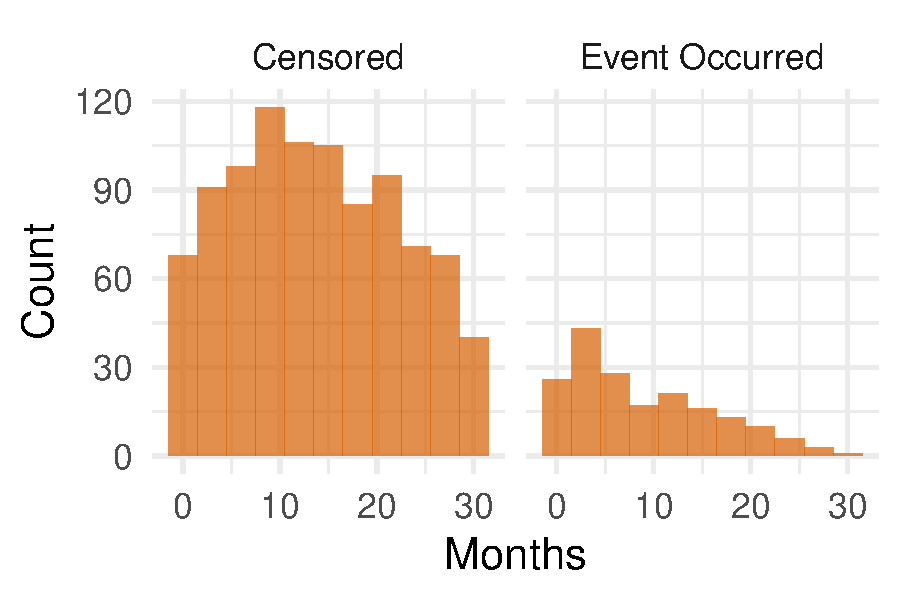
\includegraphics[height=4.5cm,width=\linewidth]{images/fake_duration_hist_a30.pdf}   % 图3路径
\caption{{\small Fake-data histogram}}
\label{fig:fake-hist_a30}
\end{subfigure}
\caption{{\small Posterior predictive checking ($A=30$).}}
\label{fig:ppc-A30}
\end{figure}

%=========================================================


\end{document}
